% =====================================================================
%  Proyecto Grupal I - Big Data (UTEC)
%  Procesamiento de Datos Masivos en la Nube
%
%  ESTRUCTURA DEL PROYECTO
%    main.tex                 -> preambulo, portada e inclusion de secciones
%    secciones/*.tex          -> una seccion del informe por archivo
%    imagenes/                -> logo y evidencia del bucket
%    imagenes/consultas/2w/   -> capturas Arquitectura A (1 master + 2 workers)
%    imagenes/consultas/4w/   -> capturas Arquitectura B (1 master + 4 workers)
%    imagenes/hadoop/         -> capturas de la practica de MapReduce
%
%  El CODIGO FUENTE no forma parte de este informe: se entrega por separado
%  en el paquete codigo-fuente (scripts de Python, notebooks y scripts de
%  Hadoop). La unica excepcion son los comandos de consola de la seccion de
%  Hadoop, que el enunciado exige incluir en el informe.
%
%  Compilar con pdfLaTeX.
% =====================================================================
\documentclass[12pt,a4paper]{article}

% ---------- Codificacion e idioma ----------
\usepackage[utf8]{inputenc}
\usepackage[T1]{fontenc}
\usepackage[spanish,es-tabla,es-noshorthands]{babel}

% ---------- Geometria y tipografia ----------
\usepackage[margin=2.5cm]{geometry}
\usepackage{lmodern}
\usepackage{microtype}
\setlength{\parskip}{0.4em}

% ---------- Matematicas ----------
\usepackage{amsmath}
\usepackage{amssymb}

% ---------- Graficos y tablas ----------
\usepackage{graphicx}
\usepackage{float}
\usepackage{booktabs}
\usepackage{longtable}
\usepackage{array}
\usepackage{multirow}
\usepackage{caption}
\usepackage{subcaption}
\usepackage{xcolor}
\usepackage{enumitem}

\graphicspath{{imagenes/}}

% ---------- Diagramas ----------
\usepackage{tikz}
\usetikzlibrary{positioning, arrows.meta, shapes.geometric, fit, backgrounds}

% ---------- Enlaces ----------
\usepackage[hidelinks]{hyperref}
\usepackage{url}
\urlstyle{same}

% ---------- Bloques de codigo ----------
\usepackage{listings}

\definecolor{codebg}{gray}{0.96}
\definecolor{codekw}{RGB}{0,0,180}
\definecolor{codecm}{RGB}{0,120,0}
\definecolor{codestr}{RGB}{200,90,0}
\definecolor{coderule}{gray}{0.75}

\lstset{
    basicstyle=\ttfamily\footnotesize,
    backgroundcolor=\color{codebg},
    frame=single,
    rulecolor=\color{coderule},
    breaklines=true,
    breakatwhitespace=false,
    showstringspaces=false,
    keywordstyle=\color{codekw}\bfseries,
    commentstyle=\color{codecm}\itshape,
    stringstyle=\color{codestr},
    numbers=left,
    numberstyle=\tiny\color{gray},
    numbersep=7pt,
    xleftmargin=2.2em,
    framexleftmargin=2em,
    captionpos=b,
    tabsize=4,
    inputencoding=utf8,
    extendedchars=true,
    literate=%
      {á}{{\'a}}1 {é}{{\'e}}1 {í}{{\'i}}1 {ó}{{\'o}}1 {ú}{{\'u}}1
      {Á}{{\'A}}1 {É}{{\'E}}1 {Í}{{\'I}}1 {Ó}{{\'O}}1 {Ú}{{\'U}}1
      {ñ}{{\~n}}1 {Ñ}{{\~N}}1 {ü}{{\"u}}1 {Ü}{{\"U}}1
      {¿}{{?`}}1 {¡}{{!`}}1 {°}{{\textdegree}}1
}

\lstdefinestyle{py}{language=Python}
\lstdefinestyle{sh}{language=bash, numbers=none}

% ---------- Ajuste fino del corte de linea ----------
% Ultimo recurso para que LaTeX estire los espacios antes de desbordar el
% margen, en lugar de sacar el texto fuera de la caja.
\setlength{\emergencystretch}{3em}
\hyphenpenalty=1000
\tolerance=2000

% \bk introduce un punto de corte de anchura cero y SIN guion. Se inserta en
% rutas y nombres largos escritos en \texttt para que puedan partirse al final
% de linea sin desbordar el margen. Es robusto dentro de tablas y pies de
% figura, a diferencia de los comandos del paquete url.
\newcommand{\bk}{\discretionary{}{}{}}

% ---------- Repositorio de codigo ----------
\newcommand{\repourl}{https://github.com/tmrainer/BigDataP1}

% \nbref{herramienta}{n}: enlaza el notebook de esa herramienta y arquitectura.
% OJO: la URL debe ir SIN \bk, o los puntos de corte acaban dentro del enlace.
% Por eso el destino y el texto mostrado se construyen por separado.
\newcommand{\nbref}[2]{%
  \href{\repourl/blob/main/notebooks/#1_#2_workers.ipynb}%
       {\texttt{notebooks/#1\_\bk{}#2\_\bk{}workers.\bk{}ipynb}}}

% Enlace a la carpeta de notebooks
\newcommand{\nbdir}{\href{\repourl/tree/main/notebooks}{\texttt{notebooks/}}}

% Linea de referencia al notebook ejecutado, bajo una consulta
\newcommand{\refnotebook}[2]{%
  \par\smallskip\noindent\footnotesize
  \textbf{Notebook ejecutado:} \nbref{#1}{#2}\par\normalsize}

% ---------- Atajos ----------
% Encabezado de bloque seguro delante de un lstlisting (un \paragraph se solapa)
\newcommand{\bloque}[1]{\par\medskip\noindent\textbf{#1}\par\nopagebreak\vspace{0.3em}}

% Figura de captura de consulta: #1 ruta  #2 pie
\newcommand{\captura}[2]{%
  \begin{figure}[htbp]
    \centering
    \includegraphics[width=0.93\textwidth]{#1}
    \caption{#2}
  \end{figure}%
}

\begin{document}

% ============================== PORTADA ==============================
\begin{titlepage}
    \centering
    \vspace*{0.5cm}

    
\includegraphics[width=0.45\textwidth]{utec-logo.jpg}\\[1cm]

    {\large Facultad de Computación}\\[0.15cm]
    {\large Ciencias de la Computación}\\[0.4cm]
    {\large Curso: Big Data}\\[1.2cm]

    {\LARGE \textbf{Proyecto Grupal I:}}\\[0.4cm]
    {\LARGE \textbf{Procesamiento de Datos Masivos en la Nube}}\\[0.6cm]
    {\large \textit{Análisis distribuido de 500,000 reseñas de Steam sobre Google Cloud Dataproc}}\\[1.8cm]

    {\large \textbf{Integrantes:}}\\[0.3cm]
    Castro Gomez, Percy Valentín \\
    Martínez Palomino, Jorge Armando \\
    Molina Álvarez, Carla Viviana \\
    Montesinos Damian, Leonardo Alberto \\
    Namihas Millan, Yitzhak Abraham \\

    \vfill

    {\large 23 de septiembre de 2026}
\end{titlepage}


\tableofcontents
\newpage

% ============================ INTRODUCCIÓN ===========================
\section{Introducción}

El presente proyecto tiene como objetivo demostrar la capacidad de gestionar grandes volúmenes de información mediante el procesamiento distribuido en la nube, utilizando los servicios de Google Cloud Platform (GCP). A través de herramientas como Polars, Dask, Modin, Apache Spark y Hadoop MapReduce, se busca procesar eficientemente un dataset masivo y generar indicadores de valor para la toma de decisiones.

El caso de estudio corresponde al dominio del comercio digital de videojuegos: se analizan 500,000 reseñas publicadas por usuarios en la plataforma Steam, con el fin de extraer métricas de satisfacción, fidelización y comportamiento de la comunidad por título. Este contexto es directamente asimilable a un escenario real de negocio de \textit{retail} digital, donde la opinión del cliente constituye un activo para decisiones de catálogo, precios y soporte.

El trabajo se estructura en cinco ejes, alineados con los requerimientos del proyecto:

\begin{enumerate}[leftmargin=*]
    \item \textbf{Fuente de datos:} descripción del origen, estructura y variables principales del conjunto de reseñas, así como el procedimiento de muestreo aplicado sobre el dataset original de más de 113 millones de registros.
    \item \textbf{Almacenamiento en la nube:} implementación de un \textit{Data Lake} sobre Google Cloud Storage, con evidencia de creación, organización de los datos y justificación de la decisión arquitectónica.
    \item \textbf{Diseño de arquitectura:} definición de dos topologías de clúster Dataproc (1 Master + 2 Workers y 1 Master + 4 Workers), con diagramas, explicación de componentes y justificación técnica.
    \item \textbf{Procesamiento distribuido:} implementación de 10 consultas equivalentes en Polars, Dask, Modin y Apache Spark, cubriendo limpieza, tratamiento de duplicados y nulos, transformación de variables, filtrado, agrupaciones, agregaciones, ordenamiento y cálculo de métricas, con medición sistemática de tiempos de ejecución.
    \item \textbf{Hadoop MapReduce:} ejecución de tres programas del archivo \texttt{hadoop-\bk{}mapreduce-\bk{}examples.\bk{}jar} (\texttt{wordmean}, \texttt{secondarysort} y \texttt{terasort}) sobre un clúster Dataproc, utilizando HDFS como sistema de archivos distribuido para la entrada y la salida.
\end{enumerate}

Un aporte diferencial de este informe es que no se limita a reportar resultados favorables. Tres hallazgos contraintuitivos se investigaron hasta su causa y se documentan con evidencia cuantitativa:

\begin{itemize}[leftmargin=*]
    \item \textbf{Duplicar el número de nodos \textit{worker} no redujo los tiempos de ejecución} en ninguna de las cuatro herramientas. Se realizó un diagnóstico empírico sobre el clúster y sobre los \textit{event logs} de Spark para identificar y comprobar las causas reales (Sección~\ref{subsec:diagnostico-spark}).
    \item \textbf{El 36.8\,\% de las filas del archivo de trabajo resultaron ser copias exactas de otras filas.} La fase de limpieza del flujo distribuido lo detectó; el análisis posterior identificó su origen en el parámetro de muestreo empleado y lo verificó con un modelo probabilístico (Sección~\ref{subsec:muestreo}).
    \item \textbf{Dos ejecuciones de MapReduce terminaron con estado \texttt{completed successfully} produciendo resultados inválidos} (\texttt{NaN} e \texttt{Infinity}). El diagnóstico mediante los contadores del \textit{job} reveló, en un caso, un archivo de entrada vacío y, en el otro, una limitación del propio programa de ejemplo frente a múltiples \textit{reducers} (Sección~\ref{subsubsec:wordmean-fallos}).
\end{itemize}

% ============================== DATASET ==============================
\section{Dataset}

\subsection{Origen y Estructura}
El conjunto de datos original, denominado \textit{100 Million+ Steam Reviews}, fue obtenido desde la plataforma Kaggle y recopilado mediante la API oficial de reseñas de usuarios de la plataforma (\textit{Steam User Reviews - Get List API}). En su versión íntegra, el dataset abarca más de 113 millones de registros históricos que capturan la interacción y opinión de los jugadores. La fuente oficial y documentación completa se encuentra disponible en: \url{https://www.kaggle.com/datasets/kieranpoc/steam-reviews/data}.

El archivo de trabajo posee un formato estructurado (CSV) y consta de 24 variables. Agrupadas por rol dentro del modelo de datos, estas son:

\begin{itemize}[leftmargin=*]
    \item \textbf{Identificadores:} \texttt{recommendationid} (ID único de la reseña), \texttt{appid} (ID del juego) y \texttt{game} (nombre del videojuego).
    \item \textbf{Perfil del jugador:} \texttt{author\_steamid} (identificador único del usuario), cantidad de juegos en su biblioteca (\texttt{author\_\bk{}num\_\bk{}games\_\bk{}owned}) y total de reseñas publicadas (\texttt{author\_num\_reviews}).
    \item \textbf{Métricas de actividad (en minutos):} tiempo de juego total histórico (\texttt{author\_\bk{}playtime\_\bk{}forever}), tiempo jugado en las últimas dos semanas (\texttt{author\_\bk{}playtime\_\bk{}last\_\bk{}two\_\bk{}weeks}), tiempo registrado al momento de escribir la reseña (\texttt{author\_\bk{}playtime\_\bk{}at\_\bk{}review}) y fecha de la última sesión (\texttt{author\_last\_played}).
    \item \textbf{Contenido e impacto de la reseña:} idioma (\texttt{language}), texto (\texttt{review}), fechas de publicación y actualización, veredicto de recomendación (\texttt{voted\_up}) y reacción de la comunidad (\texttt{votes\_up}, \texttt{votes\_funny}, \texttt{weighted\_vote\_score}, \texttt{comment\_count}).
    \item \textbf{Contexto de adquisición:} indicadores binarios que señalan si el juego fue comprado directamente en la tienda de Steam (\texttt{steam\_purchase}), si fue adquirido de forma gratuita (\texttt{received\_for\_free}) o si la reseña fue escrita durante la fase de acceso anticipado (\texttt{written\_\bk{}during\_\bk{}early\_\bk{}access}), además de las banderas de disponibilidad regional \texttt{hidden\_\bk{}in\_\bk{}steam\_\bk{}china} y \texttt{steam\_\bk{}china\_\bk{}location}.
\end{itemize}

El esquema inferido automáticamente por Polars sobre el archivo de trabajo se resume en la Tabla~\ref{tab:esquema}.

\begin{table}[H]
\centering
\caption{Esquema del dataset de trabajo (24 columnas, 500,000 registros)}
\label{tab:esquema}
\vspace{0.2cm}
\small
\begin{tabular}{llp{7.2cm}}
\toprule
\textbf{Variable} & \textbf{Tipo} & \textbf{Descripción} \\
\midrule
\texttt{recommendationid}             & Int64   & Identificador único de la reseña \\
\texttt{appid}                        & Int64   & Identificador del videojuego en Steam \\
\texttt{game}                         & String  & Nombre comercial del videojuego \\
\texttt{author\_steamid}              & Int64   & Identificador único del autor \\
\texttt{author\_\bk{}num\_\bk{}games\_\bk{}owned}    & Int64   & Juegos en la biblioteca del autor \\
\texttt{author\_num\_reviews}         & Int64   & Reseñas publicadas por el autor \\
\texttt{author\_\bk{}playtime\_\bk{}forever}    & Int64   & Minutos jugados históricos \\
\texttt{author\_\bk{}playtime\_\bk{}last\_\bk{}two\_\bk{}weeks} & Int64 & Minutos jugados en las últimas 2 semanas \\
\texttt{author\_\bk{}playtime\_\bk{}at\_\bk{}review}  & Int64  & Minutos jugados al escribir la reseña \\
\texttt{author\_last\_played}          & Int64  & \textit{Timestamp} de la última sesión \\
\texttt{language}                      & String & Idioma de la reseña \\
\texttt{review}                        & String & Texto libre de la reseña \\
\texttt{timestamp\_created}            & Int64  & \textit{Timestamp} de publicación \\
\texttt{timestamp\_updated}            & Int64  & \textit{Timestamp} de última edición \\
\texttt{voted\_up}                     & Int64  & 1 = recomienda, 0 = no recomienda \\
\texttt{votes\_up}                     & Int64  & Votos de \guillemotleft{}útil\guillemotright{} recibidos \\
\texttt{votes\_funny}                  & Int64  & Votos de \guillemotleft{}graciosa\guillemotright{} recibidos \\
\texttt{weighted\_vote\_score}         & Float64& Puntaje de utilidad ponderado por Steam \\
\texttt{comment\_count}                & Int64  & Comentarios sobre la reseña \\
\texttt{steam\_purchase}               & Int64  & 1 si el juego se compró en Steam \\
\texttt{received\_for\_free}           & Int64  & 1 si el juego se obtuvo gratis \\
\texttt{written\_\bk{}during\_\bk{}early\_\bk{}access}& Int64  & 1 si se escribió en acceso anticipado \\
\texttt{hidden\_\bk{}in\_\bk{}steam\_\bk{}china}      & Int64  & Bandera de visibilidad regional \\
\texttt{steam\_\bk{}china\_\bk{}location}        & String & Ubicación declarada (Steam China) \\
\bottomrule
\end{tabular}
\end{table}

\subsection{Selección y Preprocesamiento de Registros}
\label{subsec:muestreo}

\subsubsection{Procedimiento aplicado}

El dataset publicado en Kaggle supera los 113 millones de registros y varias decenas de gigabytes, un volumen que excede tanto el requerimiento del proyecto (mínimo 500,000 registros) como el presupuesto de cómputo asignado. Para acotar el experimento se construyó el archivo de trabajo con el siguiente procedimiento, ejecutado en Google Colab:

\begin{table}[H]
\centering
\caption{Parámetros del procedimiento de muestreo aplicado}
\label{tab:muestreo}
\vspace{0.2cm}
\small
\begin{tabular}{@{}ll@{}}
\toprule
\textbf{Parámetro} & \textbf{Valor empleado} \\
\midrule
Origen                     & Dataset \texttt{kieranpoc/\bk{}steam-\bk{}reviews} descargado con \texttt{kagglehub} \\
Archivo leído              & El primero que devuelve el listado del directorio \\
Tamaño de la muestra       & 500,000 registros \\
Tipo de muestreo           & Aleatorio \textbf{con reposición} \\
Semilla                    & 42 (reproducible) \\
Destino                    & \texttt{steam\_\bk{}reviews\_\bk{}500k.\bk{}csv} en Google Drive \\
\bottomrule
\end{tabular}
\end{table}

El archivo resultante cumple el requisito del enunciado: \textbf{500,000 registros} y 24 columnas, con un peso en disco de \textbf{700.1 MB} (667.7 MiB). Dos decisiones de ese script, sin embargo, condicionan la interpretación de los resultados y se documentan aquí de forma explícita, ya que explican por sí solas el principal hallazgo de la fase de limpieza.

\subsubsection{Caracterización empírica de la muestra}

Sobre el archivo final se midieron directamente las siguientes cantidades:

\begin{table}[H]
\centering
\caption{Estructura de unicidad del archivo de trabajo (medición directa sobre el CSV)}
\label{tab:unicidad}
\vspace{0.2cm}
\small
\begin{tabular}{lr}
\toprule
\textbf{Métrica} & \textbf{Valor} \\
\midrule
Filas del archivo                                      & 500,000 \\
Valores distintos de \texttt{recommendationid}         & 315,031 \\
Combinaciones distintas de (\texttt{author\_steamid}, \texttt{appid}, \texttt{review}) & 315,809 \\
Filas completas distintas                              & 315,809 \\
\midrule
Filas que son copia exacta de otra fila                & \textbf{184,191} \\
\bottomrule
\end{tabular}
\end{table}

El \textbf{36.8\,\%} de las filas del archivo son copias exactas de otra fila. Esta cifra no es una propiedad del dataset de origen, sino una consecuencia directa y cuantificable del muestreo con reposición.

\paragraph{Verificación del origen de los duplicados.} Al extraer $n$ elementos \textit{con reposición} de un conjunto de tamaño $N$, el número esperado de elementos distintos obtenidos es
\[
\mathbb{E}[\text{distintos}] \;=\; N\left[1-\left(1-\tfrac{1}{N}\right)^{n}\right].
\]
Con $n = 500{,}000$ y los 315,809 valores distintos observados, el tamaño implícito del conjunto de origen es $N \approx 496{,}000$ filas. La coincidencia es estrecha: para $N = 500{,}000$ la fórmula predice 316,060 filas distintas, frente a las 315,809 medidas, una desviación del 0.08\,\%.

La conclusión es doble y se verifica sin ambigüedad:

\begin{enumerate}[leftmargin=*]
    \item \textbf{El muestreo se realizó con reposición.} Si hubiera sido sin reposición, las 500,000 filas serían necesariamente distintas y no existirían duplicados exactos.
    \item \textbf{El conjunto de origen no fueron los 113 millones de registros, sino un archivo de aproximadamente 496,000 filas.} El script selecciona el primer archivo que devuelve el listado del directorio, cuyo orden depende del sistema de archivos y no del contenido; el archivo así elegido resultó ser una fracción del dataset, no su totalidad. Si el conjunto de origen hubiese tenido 113 millones de filas, el muestreo con reposición habría producido apenas unos 1,105 duplicados esperados, tres órdenes de magnitud por debajo de los 184,191 observados.
\end{enumerate}

\paragraph{Implicaciones para la validez del análisis.} Esta caracterización no invalida los resultados del proyecto, pero delimita con precisión qué se puede afirmar a partir de ellos:

\begin{itemize}[leftmargin=*]
    \item \textbf{Los indicadores calculados son válidos sobre el conjunto deduplicado.} Toda métrica del informe (tasa de recomendación, rankings, promedios) se calcula \textit{después} de la Consulta~2, es decir, sobre las 315,809 filas únicas. Esas filas son un subconjunto aleatorio del conjunto de origen, obtenido sin sesgo sistemático, por lo que las proporciones estimadas sobre ellas son estimadores insesgados de las proporciones de dicho conjunto.
    \item \textbf{La extrapolación al universo completo de Steam no está respaldada.} Como el conjunto de origen es un archivo cuya posición dentro del dataset de 113 millones no quedó documentada por el script, no puede afirmarse que sea una muestra aleatoria de la población total. Los indicadores deben leerse como propiedades de la muestra analizada, no de la plataforma completa.
    \item \textbf{La cobertura de la muestra es amplia.} Tras la limpieza se contabilizan \textbf{22,992} videojuegos distintos y reseñas en inglés, español, ruso, turco y chino simplificado, entre otros idiomas. Esto descarta que el archivo de origen corresponda a un único título, a un único idioma o a una ventana temporal estrecha, y sustenta la diversidad interna del análisis.
    \item \textbf{Los 778 registros con \texttt{recommendationid} repetido pero contenido distinto} (la diferencia entre 315,809 y 315,031) sí corresponden a un fenómeno real del origen: reediciones de una misma reseña capturadas por la API en momentos distintos.
\end{itemize}

\paragraph{Valor metodológico del hallazgo.} La detección de estos duplicados no fue un supuesto de partida, sino el resultado de la propia fase de limpieza del procesamiento distribuido: la Consulta~2 los identificó y eliminó sobre las cuatro herramientas evaluadas, con resultados idénticos entre ellas (Sección~\ref{sec:operaciones}). Este es precisamente el propósito de una etapa de validación de calidad en un flujo de Big Data, que es detectar defectos que el análisis posterior arrastraría en silencio, y constituye, en sí mismo, el indicador de calidad de datos más relevante del proyecto.

\paragraph{Corrección recomendada para trabajos futuros.} Dos cambios en el procedimiento eliminarían ambos problemas de una vez:

\begin{enumerate}[leftmargin=*]
    \item Leer la \textbf{totalidad} del dataset descargado, concatenando todos sus archivos, en lugar de únicamente el primero del listado.
    \item Muestrear \textbf{sin reposición}, de modo que las 500,000 filas resultantes sean necesariamente distintas.
\end{enumerate}

Con esos cambios, las 500,000 filas serían únicas desde el origen y la Consulta~2 reportaría 0 duplicados eliminados, confirmando la limpieza en lugar de corregir un artefacto del muestreo. El script utilizado y su versión corregida se entregan en el paquete de código fuente.

\subsubsection{Nota sobre la carga al Data Lake}

El archivo se cargó al \textit{Data Lake} en su forma cruda, sin preprocesamiento previo, de manera deliberada: toda la limpieza forma parte del procesamiento distribuido evaluado y, por tanto, del alcance medido de este proyecto. Es gracias a esa decisión que el defecto de muestreo quedó documentado con evidencia cuantitativa en lugar de pasar inadvertido.

% ========================= IMPLEMENTACIÓN GCP ========================
\section{Implementación en GCP}

\subsection{Almacenamiento en Google Cloud Storage}
Para el almacenamiento de los datos se implementó un \textit{Data Lake} utilizando un \textit{bucket} de Google Cloud Storage denominado \texttt{bigdata-2026-02}, aprovisionado en la región \texttt{us-east4} (Virginia del Norte) con clase de almacenamiento \textit{Standard}. Los datos se organizaron bajo el prefijo \texttt{proyecto01/}, que actúa como carpeta lógica del proyecto y aloja tanto el dataset de entrada como los archivos de resultados generados por los \textit{notebooks}.

\begin{table}[H]
\centering
\caption{Configuración del \textit{bucket} de Google Cloud Storage}
\label{tab:bucket}
\vspace{0.2cm}
\small
\begin{tabular}{@{}lp{9.2cm}@{}}
\toprule
\textbf{Parámetro} & \textbf{Valor} \\
\midrule
Nombre del \textit{bucket}    & \texttt{bigdata-2026-02} \\
Ubicación                     & \texttt{us-east4} (Virginia del Norte) \\
Clase de almacenamiento       & Standard \\
Acceso público                & No público \\
Protección                    & Borrado no definitivo (\textit{soft delete}) \\
Prefijo del proyecto          & \texttt{proyecto01/} \\
Objeto de entrada             & \texttt{steam\_\bk{}reviews\_\bk{}500k.\bk{}csv} (700.1 MB, \texttt{text/csv}) \\
Objetos de salida             & \texttt{tiempos\_\bk{}<herramienta>\_\bk{}<arquitectura>.\bk{}csv} (8 archivos) \\
\bottomrule
\end{tabular}
\end{table}

Como medida de seguridad, el \textit{bucket} se configuró restringiendo el acceso público a internet. Esta decisión aísla el almacenamiento y previene la exposición accidental de datos, manteniendo un canal privado dentro del mismo proyecto de GCP para que los nodos del clúster de Dataproc accedan al archivo CSV de manera interna y eficiente, a través de la cuenta de servicio del clúster.

\begin{figure}[H]
    \centering
    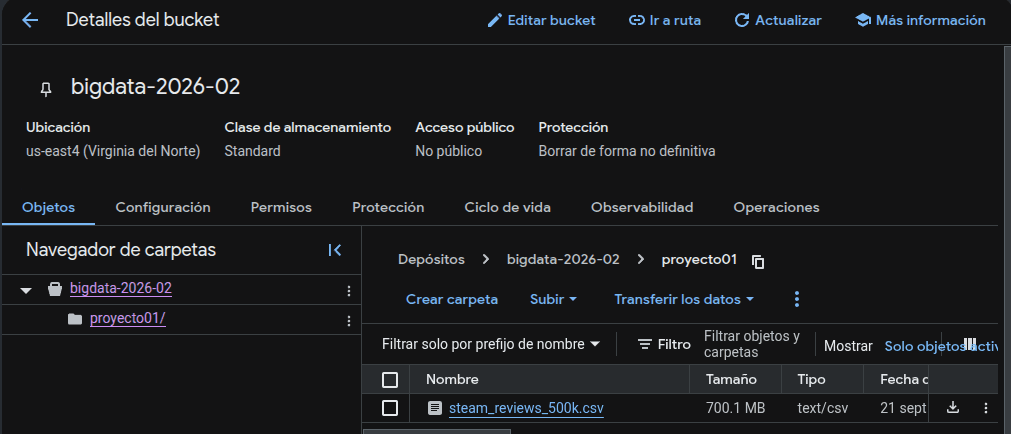
\includegraphics[width=0.9\textwidth]{bucket.png}
    \caption{Evidencia de la creación del \textit{bucket} \texttt{bigdata-2026-02}, la organización bajo el prefijo \texttt{proyecto01/} y el almacenamiento del dataset de 700.1 MB.}
    \label{fig:bucket}
\end{figure}

\subsection{Justificación del Uso de Almacenamiento en la Nube}

La decisión de emplear Google Cloud Storage como capa de almacenamiento, en lugar del disco local de las máquinas o de HDFS como repositorio permanente, responde a cuatro criterios:

\begin{itemize}[leftmargin=*]
    \item \textbf{Desacoplamiento entre almacenamiento y cómputo.} El clúster de Dataproc es un recurso \textit{efímero}: se crea para ejecutar las pruebas y se elimina al terminar, para no incurrir en costos ociosos. Si el dataset viviera en HDFS dentro del clúster, se destruiría junto con él. Al residir en GCS, el dato sobrevive a cualquier número de clústeres y permite reprovisionar la Arquitectura A o B en minutos sobre el mismo conjunto de datos, que es precisamente lo que exigió el experimento comparativo de este proyecto.
    \item \textbf{Durabilidad y disponibilidad gestionadas.} GCS ofrece redundancia y durabilidad administradas por el proveedor, sin que el equipo deba dimensionar réplicas ni gestionar fallos de disco, a diferencia del factor de replicación que habría que configurar y sostener en HDFS.
    \item \textbf{Acceso uniforme desde todos los motores.} El mismo objeto \texttt{gs:/\bk{}/\bk{}bigdata-\bk{}2026-\bk{}02/\bk{}proyecto01/\bk{}steam\_\bk{}reviews\_\bk{}500k.\bk{}csv} es consumible directamente por Spark mediante el conector de Cloud Storage, y descargable al nodo Master con \texttt{gsutil} para Polars, Dask y Modin. Un único origen de la verdad alimenta las cuatro herramientas evaluadas, lo que garantiza que la comparativa de tiempos se realice sobre datos idénticos.
    \item \textbf{Costo.} El almacenamiento de objetos tiene un costo por GB-mes sustancialmente menor que el de discos persistentes asociados a máquinas virtuales encendidas, y no requiere mantener el clúster activo para conservar los datos.
\end{itemize}

\subsection{Diseño de la Arquitectura Big Data}

La arquitectura diseñada sigue un modelo de procesamiento por lotes (\textit{batch}) nativo de la nube, separando estratégicamente el almacenamiento del poder de cómputo. El flujo abarca desde la ingesta de los datos hasta la exportación de los resultados métricos de vuelta al \textit{Data Lake}.

\subsubsection{Explicación de Componentes}
\begin{itemize}[leftmargin=*]
    \item \textbf{Fuente de datos:} dataset público \textit{100 Million+ Steam Reviews} (Kaggle), del cual se derivó la muestra de 500,000 registros descrita en la Sección~\ref{subsec:muestreo}.
    \item \textbf{Ingesta (\textit{batch}):} el archivo CSV resultante se cargó al servicio de almacenamiento de objetos de Google en una única operación de carga por lotes, sin flujo de \textit{streaming}, coherente con la naturaleza histórica y estática del conjunto.
    \item \textbf{Data Lake (almacenamiento):} \textit{bucket} \texttt{bigdata-2026-02} bajo el prefijo \texttt{proyecto01/}. Este componente actúa como repositorio central de la verdad, almacenando tanto el dataset de entrada como los archivos CSV con los tiempos de ejecución generados al finalizar cada \textit{notebook}.
    \item \textbf{Procesamiento distribuido:} clúster efímero de Google Cloud Dataproc con el componente opcional \textit{Jupyter} habilitado. El clúster monta el entorno de JupyterLab sobre el nodo Master, descarga temporalmente el dataset para las herramientas en memoria (Polars, Dask, Modin) y orquesta el procesamiento distribuido sobre YARN para Apache Spark y Hadoop MapReduce.
    \item \textbf{Salida de resultados:} cada \textit{notebook} escribe su tabla de tiempos directamente a \texttt{gs://} mediante \texttt{gcsfs}, cerrando el ciclo sobre el mismo \textit{Data Lake}.
\end{itemize}

\subsubsection{Justificación Técnica y Estrategia de Escalabilidad}
Para la validación de las herramientas se definieron instancias de segunda generación. El nodo Master emplea \texttt{n2-highmem-4} (4 vCPU, 32 GB de RAM) y los nodos \textit{worker} emplean \texttt{n2-standard-4} (4 vCPU, 16 GB de RAM). La memoria ampliada en el Master es crítica porque Polars, Dask y Modin operan sobre él de forma local: un CSV de 700 MB con una columna de texto libre de alta cardinalidad se expande varias veces en memoria al materializarse como \textit{DataFrame}, y una instancia estándar de 16 GB habría comprometido la ejecución por desbordamiento de memoria (\textit{Out of Memory}).

Para demostrar empíricamente el comportamiento del procesamiento distribuido y la escalabilidad horizontal, el proyecto evalúa dos topologías:

\begin{enumerate}[leftmargin=*]
    \item \textbf{Arquitectura A (1 Master, 2 Workers):} entorno de referencia para ejecutar y validar la correctitud de las 10 consultas en las cuatro herramientas.
    \item \textbf{Arquitectura B (1 Master, 4 Workers):} entorno ampliado, con el doble de capacidad de cómputo en los \textit{workers} (de 8 a 16 vCPU) y el mismo tipo de nodo Master, para aislar el número de \textit{workers} como única variable de estudio.
\end{enumerate}

\begin{table}[H]
\centering
\caption{Especificación de las dos topologías de clúster evaluadas}
\label{tab:clusteres}
\vspace{0.2cm}
\small
\begin{tabular}{@{}lll@{}}
\toprule
\textbf{Parámetro} & \textbf{Arquitectura A} & \textbf{Arquitectura B} \\
\midrule
Servicio                  & Cloud Dataproc          & Cloud Dataproc \\
Imagen                    & \texttt{2.3-debian12}   & \texttt{2.3-debian12} \\
Versión de Spark          & 3.5.3                   & 3.5.3 \\
Nodo Master               & 1 $\times$ \texttt{n2-highmem-4} & 1 $\times$ \texttt{n2-highmem-4} \\
\quad vCPU / RAM (Master) & 4 vCPU / 32 GB          & 4 vCPU / 32 GB \\
Nodos Worker              & 2 $\times$ \texttt{n2-standard-4} & 4 $\times$ \texttt{n2-standard-4} \\
\quad vCPU / RAM (c/u)    & 4 vCPU / 16 GB          & 4 vCPU / 16 GB \\
vCPU totales en Workers   & 8                       & 16 \\
RAM total en Workers      & 32 GB                   & 64 GB \\
Gestor de recursos        & YARN                    & YARN \\
Componente opcional       & Jupyter                 & Jupyter \\
Origen de los datos       & \multicolumn{2}{l}{\texttt{gs:/\bk{}/\bk{}bigdata-\bk{}2026-\bk{}02/\bk{}proyecto01/\bk{}}} \\
\bottomrule
\end{tabular}
\end{table}

\subsubsection{Diagramas de Arquitectura}
A continuación se presentan los diagramas de ambas topologías implementadas.

% DIAGRAMA 1: ARQUITECTURA BASE
\begin{figure}[H]
    \centering
    \begin{tikzpicture}[
        node distance=1.5cm and 2.6cm,
        box/.style={rectangle, draw=black, thick, fill=blue!10, minimum width=3cm, minimum height=1.2cm, align=center, font=\small},
        storage/.style={cylinder, draw=black, thick, aspect=0.25, fill=orange!20, minimum width=2.5cm, minimum height=3cm, shape border rotate=90, align=center, font=\small},
        arrow/.style={-{Stealth[scale=1.2]}, thick}
    ]
    \node[storage] (gcs) {Cloud Storage\\ \texttt{bigdata-2026-02}\\ \texttt{/proyecto01}};
    \node[box, right=3.2cm of gcs, fill=green!10] (master) {\textbf{Nodo Master}\\ Dataproc + Jupyter \\ (n2-highmem-4)};
    \node[box, right=2cm of master] (worker1) {\textbf{Worker 1}\\ (n2-standard-4)};
    \node[box, below=0.5cm of worker1] (worker2) {\textbf{Worker 2}\\ (n2-standard-4)};

    \draw[arrow] (gcs.15) -- node[above, font=\scriptsize, pos=0.5] {Lee datos} (master.165);
    \draw[arrow] (master.195) -- node[below, font=\scriptsize, pos=0.5] {Guarda resultados} (gcs.345);

    \draw[arrow, dashed] (master.east) -- node[above, font=\footnotesize, pos=0.55] {YARN} (worker1.west);
    \draw[arrow, dashed] (master.east) -- (worker2.west);
    \end{tikzpicture}
    \caption{Arquitectura A: clúster Dataproc con 2 nodos trabajadores.}
    \label{fig:arqA}
\end{figure}

% DIAGRAMA 2: ARQUITECTURA ESCALADA
\begin{figure}[H]
    \centering
    \begin{tikzpicture}[
        node distance=1.5cm and 2.6cm,
        box/.style={rectangle, draw=black, thick, fill=blue!10, minimum width=3cm, minimum height=1.2cm, align=center, font=\small},
        storage/.style={cylinder, draw=black, thick, aspect=0.25, fill=orange!20, minimum width=2.5cm, minimum height=3cm, shape border rotate=90, align=center, font=\small},
        arrow/.style={-{Stealth[scale=1.2]}, thick}
    ]
    \node[storage] (gcs) {Cloud Storage\\ \texttt{bigdata-2026-02}\\ \texttt{/proyecto01}};
    \node[box, right=3.2cm of gcs, fill=green!10] (master) {\textbf{Nodo Master}\\ Dataproc + Jupyter \\ (n2-highmem-4)};

    \node[box, right=2cm of master, yshift=2cm] (worker1) {\textbf{Worker 1}\\ (n2-standard-4)};
    \node[box, below=0.2cm of worker1] (worker2) {\textbf{Worker 2}\\ (n2-standard-4)};
    \node[box, below=0.2cm of worker2] (worker3) {\textbf{Worker 3}\\ (n2-standard-4)};
    \node[box, below=0.2cm of worker3] (worker4) {\textbf{Worker 4}\\ (n2-standard-4)};

    \draw[arrow] (gcs.15) -- node[above, font=\scriptsize, pos=0.5] {Lee datos} (master.165);
    \draw[arrow] (master.195) -- node[below, font=\scriptsize, pos=0.5] {Guarda resultados} (gcs.345);

    \draw[arrow, dashed] (master.east) -- (worker1.west);
    \draw[arrow, dashed] (master.east) -- (worker2.west);
    \draw[arrow, dashed] (master.east) -- (worker3.west);
    \draw[arrow, dashed] (master.east) -- (worker4.west);
    \end{tikzpicture}
    \caption{Arquitectura B: clúster Dataproc expandido a 4 nodos trabajadores para evidenciar escalabilidad horizontal.}
    \label{fig:arqB}
\end{figure}

% ====================== PROCESAMIENTO DISTRIBUIDO ====================
\section{Procesamiento Distribuido}

\subsection{Estrategia de Ejecución}
Para garantizar la estabilidad del entorno y evitar el desbordamiento de memoria RAM (\textit{Out of Memory}) en el nodo Master, la ejecución de las consultas se orquestó dividiendo el flujo de trabajo en cuatro \textit{notebooks} independientes, uno por cada tecnología: Polars, Dask, Modin y Apache Spark. Esta estrategia de aislamiento de cargas asegura que cada motor disponga del 100\,\% de los recursos asignados sin competir en segundo plano, logrando una medición de tiempos justa.

El protocolo de medición fue idéntico en los cuatro casos y en las dos arquitecturas:

\begin{enumerate}[leftmargin=*]
    \item El dataset se lee una sola vez al inicio del \textit{notebook}; esa lectura inicial \textbf{no} se contabiliza dentro de ninguna consulta.
    \item Cada consulta se cronometra con \texttt{time.time()} inmediatamente antes y después del bloque de operaciones.
    \item En los motores de evaluación diferida (\textit{lazy}), es decir Dask y Spark, cada consulta incluye explícitamente una acción de materialización (\texttt{.compute()}, \texttt{.count()} o \texttt{.show()}) dentro de la ventana cronometrada, de modo que el tiempo reportado corresponde a trabajo realmente ejecutado y no a la mera construcción del grafo de tareas.
    \item Al finalizar, los diez tiempos se consolidan en un \texttt{DataFrame} y se exportan a \texttt{gs:/\bk{}/\bk{}bigdata-\bk{}2026-\bk{}02/\bk{}proyecto01/\bk{}tiempos\_\bk{}\{framework\}\_\{arquitectura\}.csv}.
\end{enumerate}

Este último punto es relevante para la validez de la comparativa: sin una acción forzada, Dask y Spark habrían reportado tiempos cercanos a cero, no por ser más rápidos, sino por no haber ejecutado nada todavía.

\subsection{Configuración de Cada Motor}

Las cuatro herramientas se inicializaron de forma distinta, y esas diferencias son determinantes para interpretar los resultados de rendimiento. La Tabla~\ref{tab:motores} las resume; el código de inicialización de cada motor puede consultarse en su \textit{notebook} del repositorio (Tabla~\ref{tab:repo}).

\begin{table}[H]
\centering
\caption{Configuración de ejecución de cada motor}
\label{tab:motores}
\vspace{0.2cm}
\small
\begin{tabular}{@{}lp{4.2cm}p{5.2cm}@{}}
\toprule
\textbf{Motor} & \textbf{Modo de ejecución} & \textbf{Alcance en el clúster} \\
\midrule
Polars & Proceso único, paralelismo multihilo nativo (Rust) & Solo el nodo Master; lectura desde disco local tras copiar el objeto con \texttt{gsutil} \\[0.3cm]
Dask & \textit{Scheduler} distribuido sobre un \texttt{LocalCluster} & Solo el nodo Master: el cliente se instancia sin dirección de clúster, por lo que levanta trabajadores locales \\[0.3cm]
Modin & Motor Ray & Solo el nodo Master: sin el parámetro \texttt{address}, Ray crea un clúster local y no se conecta a YARN \\[0.3cm]
Apache Spark & \texttt{SparkSession} sobre YARN & \textbf{Clúster completo}: hereda \texttt{spark.master=yarn} de Dataproc y lee directamente desde \texttt{gs://} mediante el conector de Cloud Storage \\
\bottomrule
\end{tabular}
\end{table}

La consecuencia es que \textbf{solo Apache Spark ejecuta trabajo en los nodos \textit{worker}}. Polars, Dask y Modin operan íntegramente sobre el nodo Master, lo que explica por sí solo buena parte de los resultados de la Sección~\ref{sec:rendimiento}.

\paragraph{Una opción de lectura decisiva en Spark.} La lectura del CSV en Spark se configuró con \texttt{multiLine=True}. Es imprescindible para la integridad de los datos, porque el dataset contiene reseñas con saltos de línea reales dentro de campos de texto entrecomillados, y al mismo tiempo es el origen del principal cuello de botella observado. Este compromiso se analiza en la Sección~\ref{subsec:multiline}.

\subsection{Fases del Procesamiento}
El desarrollo técnico exigió la implementación de 10 consultas por herramienta, estructuradas en tres fases lógicas de ingeniería de datos:

\begin{itemize}[leftmargin=*]
    \item \textbf{Fase de exploración y limpieza (Consultas 1 a 3):} se partió de 500,000 registros. Se verificaron dimensiones, tipos de datos y valores nulos, y se realizó un tratamiento de calidad que identificó y eliminó 184,191 registros duplicados, artefactos del muestreo con reposición caracterizado en la Sección~\ref{subsec:muestreo}, dejando 315,809 registros útiles y validando la inexistencia de nulos en los campos críticos tras la limpieza.
    \item \textbf{Fase de transformación (Consultas 4 y 5):} se generó la variable derivada \texttt{review\_length} (longitud en caracteres de cada reseña) y se aplicó el filtro de veredicto positivo, que aísla 266,640 reseñas recomendadas.
    \item \textbf{Fase de análisis y métricas (Consultas 6 a 10):} se aplicaron agrupaciones, agregaciones y ordenamientos por videojuego para calcular volumen de reseñas, porcentaje de recomendación, promedio de horas jugadas, longitud media de reseña y un ranking final de títulos.
\end{itemize}

La Tabla~\ref{tab:cobertura} muestra cómo las 10 consultas cubren la totalidad de los tipos de operación exigidos por el enunciado del proyecto.

\begin{table}[H]
\centering
\caption{Cobertura de los tipos de operación requeridos}
\label{tab:cobertura}
\vspace{0.2cm}
\small
\begin{tabular}{lc}
\toprule
\textbf{Operación requerida} & \textbf{Consultas que la implementan} \\
\midrule
Limpieza de datos                        & 1, 2, 3 \\
Validación / exploración                 & 1, 3 \\
Eliminación o tratamiento de duplicados  & 2 \\
Tratamiento de valores nulos             & 3 \\
Transformación de variables              & 4 \\
Filtrado                                 & 5, 10 \\
Agrupaciones                             & 6, 7, 8, 9, 10 \\
Agregaciones                             & 6, 7, 8, 9, 10 \\
Ordenamiento                             & 6, 7, 8, 9, 10 \\
Cálculo de métricas                      & 5, 7, 8, 9, 10 \\
\bottomrule
\end{tabular}
\end{table}
\subsection{Análisis de Rendimiento}
\label{sec:rendimiento}

El aspecto más crítico del proyecto consistió en contrastar el manejo de recursos en memoria y la planificación de tareas distribuidas en el clúster Dataproc frente a un dataset de 500,000 registros. Todas las cifras que siguen provienen de los archivos CSV exportados automáticamente por los \textit{notebooks} al \textit{Data Lake} al terminar cada serie completa de diez consultas; esos CSV constituyen el registro de referencia de la medición y se entregan junto al código fuente. Las salidas visibles en los \textit{notebooks} pueden diferir puntualmente de ese registro cuando una celda se volvió a ejecutar después de la exportación, algo que ocurre en las Consultas 1 a 4 de Apache Spark sobre la Arquitectura B; las diferencias son del orden de segundos y no modifican ninguna de las conclusiones de esta sección.

\subsubsection{Resultados en la Arquitectura A (1 Master, 2 Workers)}

\begin{table}[H]
\centering
\caption{Tiempos de ejecución por consulta en la Arquitectura A (1 Master, 2 Workers)}
\label{tab:tiemposA}
\vspace{0.2cm}
\small
\begin{tabular}{lrrrr}
\toprule
\textbf{Operación} & \textbf{Polars (s)} & \textbf{Modin (s)} & \textbf{Dask (s)} & \textbf{Spark (s)} \\
\midrule
Consulta 1 (Exploración)     &   0.010 &   0.80 &  15.47 &  24.14 \\
Consulta 2 (Duplicados)      &   0.321 &   8.82 &  19.33 &  27.44 \\
Consulta 3 (Nulos)           &   0.004 &   2.17 &  49.19 &  81.98 \\
Consulta 4 (Transformar)     &   0.050 &   0.56 &  23.79 &  32.52 \\
Consulta 5 (Filtrar)         &   0.008 &   1.84 &  35.38 &  46.28 \\
Consulta 6 (Agrupación)      &   0.046 &   0.99 &  11.72 &  34.42 \\
Consulta 7 (Métricas \%)     &   0.030 &   1.25 &  12.34 &  32.73 \\
Consulta 8 (Promedios)       &   0.033 &   3.21 &  11.79 &  32.32 \\
Consulta 9 (Longitudes)      &   0.034 &   0.70 &  12.14 &  32.31 \\
Consulta 10 (Ranking)        &   0.031 &   1.12 &  12.04 &  32.84 \\
\midrule
\textbf{Total acumulado}      & \textbf{0.567} & \textbf{21.45} & \textbf{203.18} & \textbf{376.97} \\
\bottomrule
\end{tabular}
\end{table}

\paragraph{Evidencia de ejecución de las cuatro herramientas.} Las capturas siguientes muestran la misma operación, la eliminación de duplicados de la Consulta~2, resuelta por cada motor sobre el clúster. Los tres resultados coinciden en 315,809 registros y 184,191 duplicados eliminados; lo que cambia es el tiempo y, sobre todo, el modo de ejecución.

\captura{consultas/2w/modin/02.png}{Modin sobre Ray: misma operación resuelta en 8.82\,s, con el motor operando sobre el nodo Master. Notebook: \nbref{modin}{2}.}

\captura{consultas/2w/dask/05.png}{Dask: ejecución diferida con particiones sobre un \texttt{LocalCluster}, restringido al nodo Master. Notebook: \nbref{dask}{2}.}

\captura{consultas/2w/spark/02.png}{Apache Spark sobre YARN: la barra de progreso \texttt{[Stage 14: ...]} evidencia la ejecución distribuida real en los nodos \textit{worker} del clúster. Notebook: \nbref{spark}{2}.}

El orden de magnitud entre herramientas es la observación dominante: completar las diez consultas toma \textbf{0.567\,s} con Polars, \textbf{21.45\,s} con Modin, \textbf{203.18\,s} con Dask y \textbf{376.97\,s} con Apache Spark. Es decir, Spark resulta \textbf{665 veces más lento} que Polars, y Dask \textbf{358 veces} más lento, pese a ejecutar exactamente la misma lógica sobre los mismos datos y producir resultados idénticos.

El análisis por herramienta es el siguiente:

\begin{itemize}[leftmargin=*]
    \item \textbf{Polars (ejecución local optimizada).} Resolvió la totalidad de las consultas en fracciones de segundo: 0.321\,s en la eliminación de duplicados, que es la operación más costosa de su serie, y milisegundos en filtros y agregaciones. Su motor nativo en Rust, con paralelismo multihilo y representación columnar Arrow en memoria, maximiza el uso de la memoria vertical del nodo Master. Para volúmenes que caben holgadamente en la RAM física del equipo, es la opción más rápida por un margen que no admite discusión.

    \item \textbf{Modin (paralelismo sobre el Master).} Gracias a los 32 GB del nodo \texttt{n2-highmem-4}, el motor Ray subyacente completó todas las operaciones sin colapsar, con tiempos competitivos (0.556\,s en transformaciones, 8.82\,s en la deduplicación). Opera como un puente eficiente para paralelizar código de Pandas sin reescribirlo, pero depende exclusivamente del nodo Master: como se documenta en el propio \textit{notebook}, \texttt{ray.init()} sin un parámetro \texttt{address} explícito levanta un clúster de Ray local y no se conecta al gestor YARN de Dataproc.

    \item \textbf{Dask (evaluación diferida y particionado).} Al utilizar un \textit{scheduler} para manejar particiones de datos mediante un \texttt{LocalCluster} igualmente restringido al nodo Master, los tiempos se elevan de forma notable: 19.33\,s en la eliminación de duplicados y 49.19\,s en el tratamiento de nulos. El costo de orquestación de tareas (\textit{overhead}) penaliza el rendimiento en datasets de medio millón de registros, donde serializar, particionar y recomponer el dato cuesta más que procesarlo directamente.

    \item \textbf{Apache Spark (cómputo distribuido sobre YARN).} A diferencia de los frameworks anteriores, Spark sí estableció conexión real con el gestor de recursos YARN del clúster (\texttt{spark.master=yarn}), delegando trabajo a los nodos \textit{worker}. Aun así, presentó los tiempos más altos de la comparativa (de 24.14\,s a 81.98\,s por consulta). Como se detalla en la Sección~\ref{subsec:diagnostico-spark}, esto no se debe a una limitación de acceso al clúster, sino a la naturaleza de las opciones de lectura del dataset y al comportamiento adaptativo de su motor de ejecución frente a un volumen de datos comparativamente pequeño para su arquitectura.
\end{itemize}

\subsubsection{Prueba de Escalabilidad Horizontal (Arquitectura B: 1 Master, 4 Workers)}

Para validar empíricamente los beneficios del procesamiento distribuido, se provisionó una segunda arquitectura escalando el clúster a 4 nodos trabajadores (\texttt{n2-standard-4}), duplicando la capacidad de cómputo de los \textit{workers} de 8 a 16 vCPU y manteniendo el mismo tipo de nodo Master para aislar la variable de estudio.

\begin{table}[H]
\centering
\caption{Tiempos de ejecución por consulta en la Arquitectura B (1 Master, 4 Workers)}
\label{tab:tiemposB}
\vspace{0.2cm}
\small
\begin{tabular}{lrrrr}
\toprule
\textbf{Operación} & \textbf{Polars (s)} & \textbf{Modin (s)} & \textbf{Dask (s)} & \textbf{Spark (s)} \\
\midrule
Consulta 1 (Exploración)     &   0.001 &   0.64 &  16.39 &  24.53 \\
Consulta 2 (Duplicados)      &   0.318 &   8.99 &  19.77 &  26.94 \\
Consulta 3 (Nulos)           &   0.002 &   2.09 &  50.68 &  81.75 \\
Consulta 4 (Transformar)     &   0.043 &   0.59 &  23.63 &  31.91 \\
Consulta 5 (Filtrar)         &   0.010 &   5.30 &  35.87 &  46.07 \\
Consulta 6 (Agrupación)      &   0.035 &   1.36 &  12.09 &  31.13 \\
Consulta 7 (Métricas \%)     &   0.030 &   1.05 &  12.88 &  32.34 \\
Consulta 8 (Promedios)       &   0.032 &   1.10 &  12.25 &  32.23 \\
Consulta 9 (Longitudes)      &   0.044 &   0.68 &  12.35 &  31.51 \\
Consulta 10 (Ranking)        &   0.041 &   1.08 &  12.58 &  30.43 \\
\midrule
\textbf{Total acumulado}      & \textbf{0.557} & \textbf{22.90} & \textbf{208.49} & \textbf{368.82} \\
\bottomrule
\end{tabular}
\vspace{0.15cm}

{\footnotesize Fuente: los cuatro \textit{notebooks} \texttt{*\_\bk{}4\_\bk{}workers.\bk{}ipynb} de \nbdir{} en el repositorio.}
\end{table}

Los resultados arrojaron tiempos prácticamente idénticos a los de la Arquitectura A en los cuatro frameworks evaluados, como resume la Tabla~\ref{tab:comparativa}.

\begin{table}[H]
\centering
\caption{Comparativa Arquitectura A (2 Workers) frente a Arquitectura B (4 Workers): tiempo total de las 10 consultas}
\label{tab:comparativa}
\vspace{0.2cm}
\begin{tabular}{lrrrrl}
\toprule
\textbf{Herramienta} & \textbf{A (s)} & \textbf{B (s)} & \textbf{$\Delta$ (s)} & \textbf{$\Delta$ (\%)} & \textbf{\textquestiondown{}Usa los workers?} \\
\midrule
Polars & 0.567 & 0.557 & -0.011 & -1.86 & No (local al Master) \\
Modin & 21.450 & 22.899 & +1.449 & +6.75 & No (Ray local) \\
Dask & 203.176 & 208.487 & +5.311 & +2.61 & No (LocalCluster) \\
Apache Spark & 376.972 & 368.819 & -8.153 & -2.16 & Sí (YARN) \\
\bottomrule
\end{tabular}
\end{table}

Las variaciones observadas se sitúan entre $-2.16$\,\% y $+6.75$\,\%, magnitudes que corresponden al ruido normal de medición en un entorno de nube compartido (variabilidad de la red, contención de recursos del hipervisor, estado de las cachés) y no a un efecto atribuible al número de \textit{workers}. Notoriamente, Modin y Dask fueron \textit{más lentos} en la arquitectura ampliada, lo que descarta cualquier interpretación de mejora marginal.

Este comportamiento se explica por dos fenómenos de naturaleza distinta:

\begin{enumerate}[leftmargin=*]
    \item \textbf{Restricciones de ejecución local (Polars, Dask, Modin).} Las herramientas configuradas sin conexión explícita al gestor de recursos YARN levantaron clústeres locales (\texttt{LocalCluster} en Dask, instancia local de Ray en Modin) o directamente no son distribuidas (Polars). Esto limitó su ejecución a los recursos físicos del nodo Master, haciendo invisibles los nodos trabajadores adicionales de la Arquitectura B. Para estas tres herramientas, el resultado era esperable: la prueba lo confirma de forma cuantitativa.

    \item \textbf{Comportamiento adaptativo de Spark.} A diferencia de los casos anteriores, Spark sí opera sobre el clúster distribuido real vía YARN. La ausencia de mejora no se debe a una limitación de acceso, sino a un conjunto de mecanismos internos del motor de ejecución que se detallan y comprueban empíricamente en la Sección~\ref{subsec:diagnostico-spark}.
\end{enumerate}

\begin{table}[H]
\centering
\caption{Apache Spark: tiempos por consulta en ambas arquitecturas}
\label{tab:spark-ab}
\vspace{0.2cm}
\small
\begin{tabular}{lrrr}
\toprule
\textbf{Operación} & \textbf{2 Workers (s)} & \textbf{4 Workers (s)} & \textbf{Variación (s)} \\
\midrule
Consulta 1 (Exploración)     &  24.14 &  24.53 &  +0.38 \\
Consulta 2 (Duplicados)      &  27.44 &  26.94 &  -0.50 \\
Consulta 3 (Nulos)           &  81.98 &  81.75 &  -0.23 \\
Consulta 4 (Transformar)     &  32.52 &  31.91 &  -0.61 \\
Consulta 5 (Filtrar)         &  46.28 &  46.07 &  -0.21 \\
Consulta 6 (Agrupación)      &  34.42 &  31.13 &  -3.29 \\
Consulta 7 (Métricas \%)     &  32.73 &  32.34 &  -0.39 \\
Consulta 8 (Promedios)       &  32.32 &  32.23 &  -0.09 \\
Consulta 9 (Longitudes)      &  32.31 &  31.51 &  -0.80 \\
Consulta 10 (Ranking)        &  32.84 &  30.43 &  -2.41 \\
\midrule
\textbf{Total} & \textbf{376.97} & \textbf{368.82} & \textbf{-8.15} \\
\bottomrule
\end{tabular}
\end{table}

\subsubsection{Diagnóstico Empírico: \textquestiondown{}Por qué Spark no escaló?}
\label{subsec:diagnostico-spark}

A diferencia de Dask y Modin, cuya falta de escalamiento se explica por una configuración de clúster local, el caso de Spark requirió un diagnóstico más profundo, ya que sí establece conexión real con YARN. Se identificaron tres mecanismos concurrentes, verificados directamente sobre el clúster y sobre los registros de eventos (\textit{event logs}) generados por la aplicación Spark.

\paragraph{a) Lectura no paralelizable por la opción \texttt{multiLine}.}
El dataset contiene reseñas con saltos de línea reales dentro de campos de texto entre comillas, por lo que la lectura requiere la opción \texttt{multiLine=True} para no fragmentar registros incorrectamente. Esta opción, sin embargo, obliga a Spark a tratar el archivo completo como una única unidad no divisible, ya que no puede garantizar la integridad de un registro multilínea si particiona el archivo por bytes. Se verificó empíricamente:

\begin{lstlisting}[style=sh]
Particiones tras la lectura inicial (dfs.rdd.getNumPartitions()): 1
\end{lstlisting}

Es decir, la etapa de lectura y parseo del archivo de 667.7 MiB se ejecuta íntegramente en una sola tarea, sobre un único núcleo, independientemente del número de \textit{workers} disponibles en el clúster.

\paragraph{b) \textit{Adaptive Query Execution} (AQE) colapsa las particiones de \textit{shuffle}.}
Spark 3.5.3, versión desplegada por Dataproc en la imagen \texttt{2.3-debian12}, tiene activo por defecto el motor de ejecución adaptativa (\texttt{spark.\bk{}sql.\bk{}adaptive.\bk{}enabled=\bk{}true}). Aunque el clúster está configurado con \texttt{spark.\bk{}sql.\bk{}shuffle.\bk{}partitions=\bk{}1000}, AQE ajusta dinámicamente el número real de particiones tras el \textit{shuffle} en función del volumen de datos efectivamente movido. Dado que las operaciones de agregación (\texttt{groupBy}, \texttt{dropDuplicates}) sobre 500,000 registros producen resultados intermedios comparativamente pequeños, AQE fusiona las particiones nominales en un número mucho menor de particiones físicas:

\begin{lstlisting}[style=sh]
spark.sql.shuffle.partitions (configurado): 1000
Particiones reales tras groupBy("game").count(): 2
\end{lstlisting}

Este comportamiento es intencional y beneficioso en un entorno de producción con datos de tamaño variable, pero implica que, para este volumen de datos, el motor de Spark determina de forma autónoma que no se requiere más paralelismo, sin importar cuántos núcleos adicionales estén disponibles en el clúster.

\paragraph{c) \textit{Dynamic Allocation} nunca solicitó más recursos de los necesarios.}
El clúster tiene habilitada la asignación dinámica de \textit{executors} (\texttt{spark.\bk{}dynamicAllocation.\bk{}enabled=\bk{}true}, con un mínimo de 1 y un máximo de 10,000). Este mecanismo solicita nuevos \textit{executors} a YARN únicamente cuando detecta tareas en cola esperando recursos. El análisis del \textit{event log} de la aplicación \texttt{application\_\bk{}1790005002581\_\bk{}0001}, ejecutada sobre la Arquitectura B, muestra que en ningún momento se utilizaron más de 3 \textit{executors} concurrentes:

\begin{table}[H]
\centering
\caption{\textit{Executors} realmente utilizados durante la ejecución en la Arquitectura B (4 Workers)}
\label{tab:executors}
\vspace{0.2cm}
\small
\begin{tabular}{llrl}
\toprule
\textbf{Executor ID} & \textbf{Nodo Worker} & \textbf{Núcleos} & \textbf{Momento de asignación} \\
\midrule
1 & \texttt{cluster-\bk{}spark-\bk{}4w-\bk{}w-\bk{}3} & 2 & Inicio de la aplicación \\
2 & \texttt{cluster-\bk{}spark-\bk{}4w-\bk{}w-\bk{}1} & 2 & Inicio de la aplicación ($+0.1$\,s) \\
3 & \texttt{cluster-\bk{}spark-\bk{}4w-\bk{}w-\bk{}1} & 2 & $+111$\,s \\
\bottomrule
\end{tabular}
\end{table}

De los 4 nodos \textit{worker} provisionados (16 vCPU disponibles en total), la aplicación únicamente utilizó 2 nodos (\texttt{w-1} y \texttt{w-3}), con un máximo de 6 núcleos activos simultáneamente. Esto confirma que la ausencia de mejora al escalar de 2 a 4 \textit{workers} no obedece a que Spark ignore el clúster distribuido, sino a que el propio planificador de recursos, correctamente, nunca detectó una demanda de trabajo suficiente para justificar la asignación de \textit{executors} adicionales.

\paragraph{Síntesis.} Los tres mecanismos son consistentes entre sí y convergen en una misma conclusión: el volumen de trabajo por etapa, una tarea de lectura y entre 2 y 5 tareas de \textit{shuffle}, resultó insuficiente para activar el escalamiento horizontal del clúster, independientemente de la capacidad física adicional disponible en la Arquitectura B.

\subsubsection{Decisión de Diseño: Integridad de Datos frente a Paralelismo de Lectura}
\label{subsec:multiline}

Se evaluó la alternativa de omitir la opción \texttt{multiLine=True} para permitir que Spark particionara el archivo de entrada en múltiples tareas paralelas. Sin embargo, al desactivar esta opción, Spark reportó \textbf{500,027} registros en lugar de los 500,000 esperados, evidenciando que el analizador de líneas interpretó erróneamente saltos de línea contenidos dentro de campos de texto entre comillas (columna \texttt{review}) como delimitadores de nuevos registros, fragmentando y corrompiendo un número indeterminado de reseñas.

Se decidió conservar \texttt{multiLine=True} en todas las pruebas, priorizando la integridad y exactitud de los datos procesados por sobre la velocidad de la etapa de lectura. Esta decisión, si bien introduce el cuello de botella descrito en la Sección~\ref{subsec:diagnostico-spark}, se considera metodológicamente correcta: un procesamiento distribuido más rápido sobre datos corruptos no constituye un resultado válido para efectos de este proyecto. Es además la decisión que garantiza que los 184,191 duplicados detectados y los 266,640 registros positivos filtrados sean cifras comparables con las que reportan Polars, Dask y Modin.

\subsubsection{Conclusión de Escalabilidad}

La prueba demuestra que escalar horizontalmente solo produce mejoras de rendimiento cuando el volumen y la granularidad de los datos generan suficientes unidades de trabajo paralelizables para activar los mecanismos de asignación dinámica de recursos del clúster. Para un dataset de 667.7 MiB, ninguna de las cuatro tecnologías evaluadas se benefició de escalar de 2 a 4 \textit{workers}: Polars, Dask y Modin por operar de forma local al nodo Master, y Spark porque las decisiones deliberadas de integridad de datos (\texttt{multiLine=True}), combinadas con el comportamiento adaptativo del motor de ejecución (AQE y \textit{Dynamic Allocation}), resultaron en una demanda de recursos insuficiente para justificar el uso del clúster ampliado.

Esto sugiere que, para esta topología y este tamaño de dataset, la Arquitectura A constituye el punto de equilibrio óptimo entre costo y rendimiento, y que un beneficio real de la Arquitectura B solo se manifestaría ante volúmenes de datos significativamente mayores o ante una reconfiguración explícita de Spark: particionado previo del archivo de entrada (por ejemplo, a formato Parquet dividido en bloques), desactivación de AQE o asignación estática de \textit{executors}.

% ================== OPERACIONES Y RESULTADOS =========================
\section{Operaciones}
\label{sec:operaciones}

Esta sección documenta las diez operaciones implementadas sobre el dataset, con su objetivo, el tipo de operación que materializa y el resultado obtenido en la ejecución sobre Google Cloud Dataproc. Las cuatro herramientas ejecutan la \textbf{misma lógica} sobre los \textbf{mismos datos}, y esa equivalencia se verificó consulta por consulta: es el requisito que hace comparables los tiempos de la Sección~\ref{sec:rendimiento}.

La verificación arrojó coincidencia exacta en las Consultas 1 a 5 y en la 10, y \textbf{una única divergencia sistemática} en las Consultas 6 a 9, documentada en la Sección~\ref{subsec:divergencia}. No se trata de un error de implementación, sino de una diferencia de semántica entre las API que resulta instructiva por sí misma.

Cada consulta se acompaña de la captura de su ejecución en el entorno de JupyterLab del clúster. Las capturas corresponden a la implementación en Polars sobre la Arquitectura A, por ser la de salida más legible; la Sección~\ref{sec:rendimiento} incluye las evidencias equivalentes de Dask, Modin y Apache Spark.

Bajo cada consulta se indica el \textit{notebook} del repositorio donde puede consultarse su código y su salida completa. Las implementaciones equivalentes en las otras tres herramientas están en los archivos que lista la Tabla~\ref{tab:repo}.

\begin{table}[H]
\centering
\caption{Resumen de las 10 operaciones implementadas y su resultado principal}
\label{tab:resumen-consultas}
\vspace{0.2cm}
\small
\begin{tabular}{clp{7.4cm}}
\toprule
\textbf{\#} & \textbf{Operación} & \textbf{Resultado principal} \\
\midrule
1  & Exploración         & 500,000 filas $\times$ 24 columnas; nulos solo en \texttt{game} (35) y \texttt{steam\_\bk{}china\_\bk{}location} (499,985) \\
2  & Duplicados          & 184,191 duplicados eliminados; quedan 315,809 registros \\
3  & Nulos               & 0 registros eliminados: \texttt{review} está 100\,\% poblada \\
4  & Transformación      & Variable \texttt{review\_length} creada sobre 315,809 registros \\
5  & Filtrado            & 266,640 reseñas positivas; tasa global de recomendación 84.43\,\% \\
6  & Agrupación          & 22,992 juegos; Counter-Strike 2 lidera con 1,923 reseñas \\
7  & Métrica \%          & 22,992 juegos; el \textit{top} por \% lo ocupan títulos con 1--4 reseñas \\
8  & Promedios           & Máximo de 2.18 M minutos promedio; dominado por valores atípicos \\
9  & Longitudes          & Techo de 8,000 caracteres: límite impuesto por Steam \\
10 & Ranking             & 609 juegos con $\geq$ 100 reseñas; Left 4 Dead 2 lidera con 100\,\% \\
\bottomrule
\end{tabular}
\end{table}


\subsection{Consulta 1: Exploración y validación del dataset}

\textbf{Tipo de operación:} Validación / exploración.

\textbf{Objetivo:} Conocer dimensiones, estructura, tipos de datos y conteo de valores nulos del dataset crudo.

\captura{consultas/2w/polars/01.png}{Ejecución y resultado de la Consulta 1 (Exploración y validación del dataset) en el clúster de Dataproc.}

\paragraph{Resultado.}
El dataset crudo contiene \textbf{500,000 filas} y \textbf{24 columnas}. La inferencia de tipos asignó \texttt{Int64} a las 19 variables numéricas, \texttt{Float64} a \texttt{weighted\_vote\_score} y \texttt{String} a \texttt{game}, \texttt{language}, \texttt{review} y \texttt{steam\_\bk{}china\_\bk{}location}.

El conteo de nulos reveló dos hallazgos relevantes: \texttt{game} presenta \textbf{35} valores faltantes, que corresponden a títulos retirados del catálogo cuyo nombre la API ya no resuelve, y \texttt{steam\_\bk{}china\_\bk{}location} presenta \textbf{499,985} nulos, es decir, está vacía en el 99.997\,\% de los registros. Las 22 columnas restantes no registran ningún valor nulo. Se concluye que \texttt{steam\_\bk{}china\_\bk{}location} no aporta información analítica y que la calidad del resto del conjunto es alta.

\paragraph{Tiempos de ejecución (Arquitectura A).}
Polars 0.010\,s \textbar{} Modin 0.805\,s \textbar{} Dask 15.47\,s \textbar{} Spark 24.14\,s.

\refnotebook{polars}{2}


\subsection{Consulta 2: Eliminación de duplicados}

\textbf{Tipo de operación:} Tratamiento de duplicados.

\textbf{Objetivo:} Eliminar registros repetidos considerando la terna (\texttt{author\_steamid}, \texttt{appid}, \texttt{review}).

\captura{consultas/2w/polars/02.png}{Ejecución y resultado de la Consulta 2 (Eliminación de duplicados) en el clúster de Dataproc.}

\paragraph{Resultado.}
Se eliminaron \textbf{184,191} registros duplicados (36.8\,\% del total), pasando de \textbf{500,000} a \textbf{315,809} registros únicos. Las cuatro herramientas devolvieron exactamente el mismo resultado, lo que valida su equivalencia funcional y descarta que las diferencias de tiempo posteriores provengan de trabajos distintos.

\textbf{Origen de los duplicados.} Como se demuestra en la Sección~\ref{subsec:muestreo}, estos registros \textbf{no} son reediciones capturadas por la API de Steam, sino copias exactas introducidas por el muestreo con reposición que construyó el archivo de trabajo. La medición directa sobre el CSV lo confirma: las 315,809 combinaciones distintas de la clave coinciden exactamente con el número de filas completas distintas del archivo.

\textbf{Sobre la elección de la clave.} Se deduplicó por la terna en lugar de por \texttt{recommendationid}. El archivo contiene 315,031 valores distintos de ese identificador frente a 315,809 combinaciones distintas de la terna: los \textbf{778} registros de diferencia son reediciones reales de una misma reseña capturadas en momentos distintos. La clave compuesta las conserva como observaciones independientes; una deduplicación por identificador técnico las habría colapsado.

\paragraph{Tiempos de ejecución (Arquitectura A).}
Polars 0.321\,s \textbar{} Modin 8.82\,s \textbar{} Dask 19.33\,s \textbar{} Spark 27.44\,s.

\refnotebook{polars}{2}


\subsection{Consulta 3: Tratamiento de valores nulos}

\textbf{Tipo de operación:} Limpieza de datos.

\textbf{Objetivo:} Identificar valores faltantes tras la deduplicación y eliminar registros sin contenido en \texttt{review}.

\captura{consultas/2w/polars/03.png}{Ejecución y resultado de la Consulta 3 (Tratamiento de valores nulos) en el clúster de Dataproc.}

\paragraph{Resultado.}
Sobre los 315,809 registros deduplicados, el recuento de nulos quedó en \textbf{22} para \texttt{game} y \textbf{315,797} para \texttt{steam\_\bk{}china\_\bk{}location}; el resto de columnas, incluida \texttt{review}, sin nulos.

En consecuencia, la eliminación de registros sin reseña descartó \textbf{0} filas y el conjunto se mantuvo en \textbf{315,809}. Lejos de ser un resultado vacío, este es el criterio de validación buscado: confirma que la variable central del análisis está íntegramente poblada y que ningún indicador posterior se calcula sobre contenido faltante.

\paragraph{Tiempos de ejecución (Arquitectura A).}
Polars 0.004\,s \textbar{} Modin 2.17\,s \textbar{} Dask 49.19\,s \textbar{} Spark 81.98\,s.

\refnotebook{polars}{2}


\subsection{Consulta 4: Transformación de variables}

\textbf{Tipo de operación:} Transformación de variables.

\textbf{Objetivo:} Crear la variable derivada \texttt{review\_length} con la cantidad de caracteres de cada reseña.

\captura{consultas/2w/polars/04.png}{Ejecución y resultado de la Consulta 4 (Transformación de variables) en el clúster de Dataproc.}

\paragraph{Resultado.}
Se generó \texttt{review\_length} sobre los \textbf{315,809} registros limpios. Los valores observados en la muestra de control abarcan desde reseñas de 48 y 49 caracteres hasta textos de 1,104 caracteres, confirmando la alta dispersión de la variable.

Esta nueva característica habilita la Consulta~9 y, en términos de negocio, funciona como aproximación al grado de elaboración de la opinión: las reseñas extensas tienden a corresponder a jugadores con mayor tiempo invertido en el título.

\paragraph{Tiempos de ejecución (Arquitectura A).}
Polars 0.050\,s \textbar{} Modin 0.556\,s \textbar{} Dask 23.79\,s \textbar{} Spark 32.52\,s.

\refnotebook{polars}{2}


\subsection{Consulta 5: Filtrado de reseñas recomendadas}

\textbf{Tipo de operación:} Filtrado y cálculo de métricas.

\textbf{Objetivo:} Seleccionar los registros con veredicto positivo (\texttt{voted\_up} = 1) y calcular la tasa global de recomendación.

\captura{consultas/2w/polars/05.png}{Ejecución y resultado de la Consulta 5 (Filtrado de reseñas recomendadas) en el clúster de Dataproc.}

\paragraph{Resultado.}
De los \textbf{315,809} registros limpios, \textbf{266,640} corresponden a reseñas positivas, lo que arroja una \textbf{tasa global de recomendación del 84.43\,\%}.

Este es el primer indicador de valor del proyecto: en la muestra analizada, cinco de cada seis reseñas son favorables. El dato fija la línea base contra la cual debe compararse cualquier título individual: un juego con 80\,\% de recomendación está por debajo de la media de la muestra, no por encima, pese a que el valor absoluto parezca alto.

\paragraph{Tiempos de ejecución (Arquitectura A).}
Polars 0.008\,s \textbar{} Modin 1.84\,s \textbar{} Dask 35.38\,s \textbar{} Spark 46.28\,s.

\refnotebook{polars}{2}


\subsection{Consulta 6: Cantidad de reseñas por videojuego}

\textbf{Tipo de operación:} Agrupación, agregación y ordenamiento.

\textbf{Objetivo:} Agrupar por \texttt{game} y contar el total de reseñas por título, ordenando de mayor a menor.

\captura{consultas/2w/polars/06.png}{Ejecución y resultado de la Consulta 6 (Cantidad de reseñas por videojuego) en el clúster de Dataproc.}

\paragraph{Resultado.}
La agrupación procesó \textbf{22,992} videojuegos distintos en Polars y Apache Spark, y \textbf{22,991} en Dask y Modin. Esa diferencia de una unidad es sistemática, tiene una causa identificada y se analiza en la Sección~\ref{subsec:divergencia}. El \textit{Top 10} por volumen lo encabezan \textit{Counter-Strike 2} (1,923 reseñas), \textit{PUBG: BATTLEGROUNDS} (1,513), \textit{Stardew Valley} (1,413), \textit{Terraria} (1,264) y \textit{The Witcher 3: Wild Hunt} (1,228).

El resultado valida la representatividad interna de la muestra: los títulos más reseñados coinciden con los superventas históricos de la plataforma. Además, con 22,992 juegos y un máximo de 1,923 reseñas, se evidencia una distribución de cola larga extrema, en la que el título más popular concentra apenas el 0.6\,\% de las reseñas.

\paragraph{Tiempos de ejecución (Arquitectura A).}
Polars 0.046\,s \textbar{} Modin 0.991\,s \textbar{} Dask 11.72\,s \textbar{} Spark 34.42\,s.

\refnotebook{polars}{2}


\subsection{Consulta 7: Porcentaje de recomendación por videojuego}

\textbf{Tipo de operación:} Agrupación, agregación múltiple y métrica derivada.

\textbf{Objetivo:} Calcular, por juego, el total de reseñas, el total de reseñas positivas y el porcentaje de recomendación.

\captura{consultas/2w/polars/07.png}{Ejecución y resultado de la Consulta 7 (Porcentaje de recomendación por videojuego) en el clúster de Dataproc.}

\paragraph{Resultado.}
Se calculó el indicador sobre los \textbf{22,992} juegos. El ordenamiento directo por porcentaje descendente resultó, sin embargo, \textbf{analíticamente inútil}: las diez primeras posiciones están ocupadas por títulos con 100\,\% de recomendación pero con entre \textbf{1 y 4 reseñas} en total.

Este hallazgo es metodológicamente valioso: un porcentaje calculado sobre una sola observación no es una medida de calidad, sino ruido estadístico. Es precisamente la razón por la cual la Consulta~10 incorpora un umbral mínimo de volumen antes de construir el ranking definitivo.

\paragraph{Tiempos de ejecución (Arquitectura A).}
Polars 0.030\,s \textbar{} Modin 1.25\,s \textbar{} Dask 12.34\,s \textbar{} Spark 32.73\,s.

\refnotebook{polars}{2}


\subsection{Consulta 8: Promedio de horas jugadas por videojuego}

\textbf{Tipo de operación:} Agrupación, agregación (media) y ordenamiento.

\textbf{Objetivo:} Calcular el promedio de \texttt{author\_\bk{}playtime\_\bk{}forever} por juego, como aproximación a la fidelización.

\captura{consultas/2w/polars/08.png}{Ejecución y resultado de la Consulta 8 (Promedio de horas jugadas por videojuego) en el clúster de Dataproc.}

\paragraph{Resultado.}
Se procesaron los \textbf{22,992} juegos. Los valores máximos alcanzan promedios de \textbf{2.18 millones de minutos}, más de 36,000 horas, para títulos prácticamente desconocidos.

La interpretación correcta de estas cifras no es «son los juegos más adictivos». Se trata de títulos con muy pocas reseñas en la muestra, cuyos autores mantienen Steam abierto de forma permanente o usan software que deja el contador activo en segundo plano. El promedio simple, sin ponderar por número de observaciones ni acotar valores atípicos, es altamente sensible a estos casos extremos: ese es el segundo hallazgo metodológico del análisis.

\paragraph{Tiempos de ejecución (Arquitectura A).}
Polars 0.033\,s \textbar{} Modin 3.21\,s \textbar{} Dask 11.79\,s \textbar{} Spark 32.32\,s.

\refnotebook{polars}{2}


\subsection{Consulta 9: Longitud promedio de reseñas por videojuego}

\textbf{Tipo de operación:} Agrupación, agregación (media) y ordenamiento.

\textbf{Objetivo:} Calcular el promedio de \texttt{review\_length} agrupado por \texttt{game}.

\captura{consultas/2w/polars/09.png}{Ejecución y resultado de la Consulta 9 (Longitud promedio de reseñas por videojuego) en el clúster de Dataproc.}

\paragraph{Resultado.}
Se procesaron los \textbf{22,992} juegos. El ordenamiento descendente revela un techo nítido en \textbf{8,000.0} caracteres exactos, compartido por varios títulos, seguido de valores de 7,999 y 7,998.

Este patrón no es casual: refleja el \textbf{límite de 8,000 caracteres} que impone Steam al texto de una reseña. Los primeros puestos corresponden, por tanto, a juegos con una única reseña que llega al tope permitido. La detección de este techo artificial es un ejemplo directo de validación de datos: sin este análisis, la variable podría interpretarse erróneamente como una medida continua sin cota superior.

\paragraph{Tiempos de ejecución (Arquitectura A).}
Polars 0.034\,s \textbar{} Modin 0.702\,s \textbar{} Dask 12.14\,s \textbar{} Spark 32.31\,s.

\refnotebook{polars}{2}


\subsection{Consulta 10: Ranking final de videojuegos}

\textbf{Tipo de operación:} Agrupación, agregación, filtrado y ordenamiento múltiple.

\textbf{Objetivo:} Construir el ranking definitivo combinando porcentaje de recomendación y volumen, exigiendo un mínimo de 100 reseñas por título.

\captura{consultas/2w/polars/10.png}{Ejecución y resultado de la Consulta 10 (Ranking final de videojuegos) en el clúster de Dataproc.}

\paragraph{Resultado.}
Tras aplicar el umbral de \textbf{100 reseñas mínimas}, el universo se reduce de 22,992 a \textbf{609} videojuegos estadísticamente comparables. Encabezan el ranking \textit{Left 4 Dead 2} (821 reseñas, 100\,\% positivas), \textit{Subnautica} (807, 100\,\%), \textit{Mirror} (604) y \textit{Plants vs. Zombies: Game of the Year} (532).

Este sí constituye un indicador accionable: a diferencia del resultado de la Consulta~7, aquí el 100\,\% de recomendación está respaldado por cientos de observaciones independientes. El ordenamiento secundario por volumen resuelve los empates en el porcentaje, que de otro modo serían arbitrarios.

Resulta además significativo que el corte de 100 reseñas descarte al 97.4\,\% de los títulos (22,383 de 22,992): la conclusión de negocio es que, en un catálogo de cola larga como el de Steam, cualquier tablero de indicadores basado en porcentajes debe incorporar un umbral de volumen para no quedar dominado por el ruido.

\paragraph{Tiempos de ejecución (Arquitectura A).}
Polars 0.031\,s \textbar{} Modin 1.12\,s \textbar{} Dask 12.04\,s \textbar{} Spark 32.84\,s.

\refnotebook{polars}{2}


\subsection{Divergencia entre Herramientas: el Tratamiento de Claves Nulas}
\label{subsec:divergencia}

La verificación cruzada de los resultados reveló una discrepancia constante en las Consultas 6 a 9, las que agrupan por videojuego. El número de grupos obtenido no es el mismo en las cuatro herramientas.

\begin{table}[H]
\centering
\caption{Grupos obtenidos al agrupar por \texttt{game}, por herramienta y consulta}
\label{tab:divergencia}
\vspace{0.2cm}
\small
\begin{tabular}{@{}lcccc@{}}
\toprule
\textbf{Herramienta} & \textbf{Consulta 6} & \textbf{Consulta 7} & \textbf{Consulta 8} & \textbf{Consulta 9} \\
\midrule
Polars        & 22,992 & 22,992 & 22,992 & 22,992 \\
Apache Spark  & 22,992 & 22,992 & 22,992 & 22,992 \\
Dask          & 22,991 & 22,991 & 22,992 & 22,992 \\
Modin         & 22,991 & 22,991 & 22,991 & 22,991 \\
\bottomrule
\end{tabular}
\end{table}

\paragraph{Causa.} La diferencia procede del tratamiento por defecto de las claves nulas en la operación de agrupamiento, y no de ningún error en la lógica implementada:

\begin{itemize}[leftmargin=*]
    \item \texttt{groupby()} de \textbf{pandas}, y por herencia el de \textbf{Modin} y \textbf{Dask}, aplica \texttt{dropna=True} por defecto: \textbf{descarta} las filas cuya clave de agrupamiento es nula.
    \item \texttt{group\_by()} de \textbf{Polars} y \texttt{groupBy()} de \textbf{Apache Spark} \textbf{conservan} el valor nulo como un grupo más.
\end{itemize}

La Consulta~3 había documentado que, tras la deduplicación, la columna \texttt{game} conserva \textbf{22 valores nulos}, correspondientes a títulos retirados del catálogo cuyo nombre la API ya no resuelve. Esas 22 filas forman un único grupo adicional bajo la semántica de Polars y Spark, lo que explica con exactitud la unidad de diferencia: $22{,}991 + 1 = 22{,}992$.

\paragraph{Por qué Dask coincide en las Consultas 8 y 9.} Dask reporta 22,992 en las agregaciones de media (\texttt{mean}) pese a usar la semántica de pandas. El motivo es que su planificador calcula esas agregaciones por particiones y recompone el resultado en una etapa final, en la que el grupo nulo reaparece en el índice. Es un detalle de implementación de su motor diferido, no una diferencia de criterio.

\paragraph{Implicaciones.} El efecto sobre los indicadores del proyecto es nulo en términos prácticos: las 22 filas afectadas representan el 0.007\,\% de los 315,809 registros limpios y no alteran ninguna de las posiciones del \textit{Top 10} ni del ranking final, donde el umbral de 100 reseñas las excluye de todos modos. Las cuatro herramientas devuelven \textbf{609} videojuegos en la Consulta~10.

El hallazgo es, sin embargo, relevante desde el punto de vista de la ingeniería de datos. Demuestra que \textbf{migrar una carga de trabajo entre motores no es una operación neutra}: dos implementaciones sintácticamente equivalentes pueden diferir en el valor por defecto de un parámetro y producir resultados distintos sin emitir ninguna advertencia. En un entorno de producción, donde la columna de agrupamiento podría tener un porcentaje de nulos mucho mayor, esta discrepancia silenciosa sería una fuente real de error. La forma de eliminarla es explicitar el criterio en lugar de confiar en el valor por defecto, fijando \texttt{dropna=False} en las herramientas basadas en pandas.

\subsection{Indicadores de Valor Generados}

A partir del procesamiento distribuido se extrajeron los siguientes indicadores sobre el comportamiento de la comunidad de Steam en la muestra analizada:

\begin{enumerate}[leftmargin=*]
    \item \textbf{Tasa global de recomendación: 84.43\,\%.} De 315,809 reseñas limpias, 266,640 son positivas. Este valor constituye la línea base contra la cual debe evaluarse cualquier título individual dentro de la muestra.
    \item \textbf{Defecto de muestreo detectado y cuantificado: 36.8\,\% del archivo.} Uno de cada tres registros del archivo de trabajo es copia exacta de otro (Sección~\ref{subsec:muestreo}). El valor del hallazgo no es el dato en sí, sino que la fase de limpieza lo detectó de forma autónoma: cualquier tablero construido sobre el dato crudo habría sobreestimado el volumen de opiniones en más de un tercio sin emitir ninguna señal de error.
    \item \textbf{Concentración del catálogo: 2.6\,\%.} Solo 609 de 22,992 videojuegos alcanzan las 100 reseñas. El catálogo es de cola larga extrema, y las métricas porcentuales requieren umbrales de volumen para ser interpretables.
    \item \textbf{Ranking de fidelización.} \textit{Left 4 Dead 2} (821 reseñas, 100\,\% positivas) y \textit{Subnautica} (807, 100\,\%) encabezan el ranking de títulos con respaldo estadístico suficiente.
    \item \textbf{Límite estructural de la variable de texto: 8,000 caracteres.} Detectado empíricamente en la Consulta~9; condiciona cualquier análisis futuro de extensión o de procesamiento de lenguaje natural sobre este campo.
\end{enumerate}

% ============================== HADOOP ===============================
\section{Hadoop MapReduce en Google Cloud Dataproc}
\label{sec:hadoop}

Esta sección documenta la ejecución de tres programas del archivo \texttt{hadoop-\bk{}mapreduce-\bk{}examples.\bk{}jar} sobre un clúster administrado de Google Cloud Dataproc, utilizando HDFS como sistema de archivos distribuido tanto para la entrada como para la salida. Conforme al enunciado, se excluyeron los programas \texttt{wordcount} y \texttt{grep}. Los programas seleccionados fueron \texttt{wordmean}, \texttt{secondarysort} y \texttt{terasort}, elegidos por cubrir tres perfiles de carga distintos: cálculo estadístico sobre texto, control del comportamiento interno del framework, y \textit{benchmark} de ordenamiento distribuido a escala.

\subsection{Entorno de Ejecución}

Esta fase se ejecutó sobre un clúster independiente del utilizado en las Secciones~\ref{sec:operaciones} y~\ref{sec:rendimiento}, provisionado específicamente para la práctica de MapReduce.

\begin{table}[H]
\centering
\caption{Configuración del clúster utilizado para Hadoop MapReduce}
\label{tab:hadoop-cluster}
\vspace{0.2cm}
\small
\begin{tabular}{@{}ll@{}}
\toprule
\textbf{Componente} & \textbf{Configuración} \\
\midrule
Servicio                & Google Cloud Dataproc \\
Proyecto                & \texttt{eco-\bk{}tenure-\bk{}506905-\bk{}q7} \\
Clúster                 & \texttt{cluster-bigdata-v2} \\
Región                  & \texttt{us-east4} (\textit{auto zone placement}) \\
Imagen                  & \texttt{2.3-debian12} \\
Versión de Hadoop       & Apache Hadoop \textbf{3.3.6} \\
Nodo maestro            & 1 $\times$ \texttt{n2-highmem-4}, disco 50 GB \\
Workers                 & 2 $\times$ \texttt{n2-standard-4}, disco 50 GB \\
Componentes opcionales  & JupyterLab + Component Gateway \\
Bucket de \textit{staging} & \texttt{bigdata-2026-02} \\
JAR utilizado           & \texttt{/\bk{}usr/\bk{}lib/\bk{}hadoop-\bk{}mapreduce/\bk{}hadoop-\bk{}mapreduce-\bk{}examples.\bk{}jar} \\
\bottomrule
\end{tabular}
\end{table}

\paragraph{Sobre el JAR de ejemplos.} El archivo \texttt{hadoop-\bk{}mapreduce-\bk{}examples.\bk{}jar} viene preinstalado en cada nodo del clúster como parte de la distribución de Hadoop; no fue necesario descargarlo de Maven Central ni subirlo manualmente. Al inspeccionarlo se comprobó que se trata de un enlace simbólico:

\begin{lstlisting}[style=sh]
lrwxrwxrwx 1 root root 35 Aug 30 07:20
/usr/lib/hadoop-mapreduce/hadoop-mapreduce-examples.jar
    -> hadoop-mapreduce-examples-3.3.6.jar
\end{lstlisting}

Esa indirección es la que permite confirmar la versión exacta de Hadoop del clúster. Ejecutar el JAR sin argumentos lista los programas disponibles, de donde se seleccionaron los tres de esta práctica.

\paragraph{Acceso al clúster.} Todos los comandos se ejecutaron en el nodo maestro (\texttt{cluster-\bk{}bigdata-\bk{}v2-\bk{}m}) a través de la terminal de JupyterLab, habilitada gracias a \texttt{-\bk{}-\bk{}optional-\bk{}components=\bk{}JUPYTER} y \texttt{-\bk{}-\bk{}enable-\bk{}component-\bk{}gateway}. Es funcionalmente equivalente a conectarse con \texttt{gcloud compute ssh}, con la diferencia de que la sesión corre como usuario \texttt{root}. Por ese motivo se optó por rutas fijas en HDFS (\texttt{/tarea/...}) en lugar de \texttt{/user/\$(whoami)/...}, evitando inconsistencias entre sesiones.

\begin{lstlisting}[style=sh, caption={Creación del clúster}]
gcloud dataproc clusters create cluster-bigdata-v2 \
    --region=us-east4 \
    --subnet=default \
    --master-machine-type=n2-highmem-4 \
    --master-boot-disk-size=50GB \
    --num-workers=2 \
    --worker-machine-type=n2-standard-4 \
    --worker-boot-disk-size=50GB \
    --image-version=2.3-debian12 \
    --optional-components=JUPYTER \
    --enable-component-gateway \
    --bucket=bigdata-2026-02
\end{lstlisting}

\captura{hadoop/00_entorno/03_jar_symlink_hadoop_336.png}{Verificación del JAR de ejemplos: el enlace simbólico revela la versión Apache Hadoop 3.3.6 del clúster.}

\captura{hadoop/00_entorno/04_lista_programas_disponibles.png}{Listado de los programas incluidos en \texttt{hadoop-\bk{}mapreduce-\bk{}examples.\bk{}jar}, de donde se seleccionaron los tres de esta práctica.}

\begin{table}[H]
\centering
\caption{Resumen de los tres programas MapReduce ejecutados}
\label{tab:hadoop-resumen}
\vspace{0.2cm}
\small
\begin{tabular}{@{}llrrr@{}}
\toprule
\textbf{Programa} & \textbf{Dataset de entrada} & \textbf{Volumen} & \textbf{Mappers} & \textbf{Reducers} \\
\midrule
\texttt{wordmean}      & Don Quijote (Project Gutenberg) & 2.1 MB    & 1  & 1 \\
\texttt{secondarysort} & MovieLens 100K (GroupLens)      & 779 KB    & 1  & 1 \\
\texttt{teragen}       & Generado sintéticamente         & 100 MB    & 21 & 0 \\
\texttt{terasort}      & Salida de \texttt{teragen}      & 100 MB    & 21 & 7 \\
\bottomrule
\end{tabular}
\end{table}

% =====================================================================
\subsection{Programa 1: \texttt{wordmean}}

\paragraph{Objetivo.} Calcular la longitud promedio de las palabras de un conjunto de archivos de texto. En la fase \textit{Map}, cada palabra emite dos pares clave-valor: uno con la clave \texttt{count} (valor 1) y otro con la clave \texttt{length} (valor igual al número de caracteres de la palabra). En la fase \textit{Reduce} se suman ambos acumuladores. Finalmente el propio programa lee el archivo de salida y divide \texttt{length}/\texttt{count} para imprimir la media en consola. Comparte la estructura de \texttt{wordcount} (tokenización de texto) pero produce un resultado estadístico en lugar de un simple conteo.

\paragraph{Dataset de entrada y justificación.} Se utilizó \textbf{\guillemotleft{}Don Quijote de la Mancha\guillemotright{}} (Project Gutenberg, eBook \#2000), en texto plano UTF-8. La primera opción fueron los archivos \texttt{LICENSE.txt} y \texttt{NOTICE.txt} que vienen con cualquier instalación de Hadoop, pero se descartaron por ser textos legales, de tamaño pequeño y poco representativos como conjunto de datos en un contexto de Big Data. El Quijote se eligió por tres razones: es obra de \textbf{dominio público}, citable sin restricciones de licencia; está disponible en \textbf{UTF-8}, exactamente el formato que espera \texttt{TextInputFormat} de Hadoop, de modo que las tildes y la \guillemotleft{}ñ\guillemotright{} se procesan sin configuración adicional; y es texto natural real, con gran variedad léxica, por lo que la media calculada tiene una interpretación lingüística genuina. Se recortaron la cabecera y el pie legal que Project Gutenberg añade a todos sus archivos, para que la estadística refleje únicamente el texto de la novela.

\bloque{Comando ejecutado.}
\begin{lstlisting}[style=sh]
JAR=/usr/lib/hadoop-mapreduce/hadoop-mapreduce-examples.jar

# 1. Descarga y limpieza del texto
wget -O ~/datos/quijote.txt https://www.gutenberg.org/ebooks/2000.txt.utf-8
sed -n '/START OF THE PROJECT GUTENBERG/,/END OF THE PROJECT GUTENBERG/p' \
    ~/datos/quijote.txt > ~/datos/quijote_limpio.txt
wc -l ~/datos/quijote_limpio.txt          # verificacion: ~37,683 lineas

# 2. Carga en HDFS
hdfs dfs -mkdir -p /tarea/wordmean/input
hdfs dfs -put -f ~/datos/quijote_limpio.txt /tarea/wordmean/input/

# 3. Ejecucion del job (ver 7.3.1 sobre -D mapreduce.job.reduces=1)
hdfs dfs -rm -r -f -skipTrash /tarea/wordmean/output
hadoop jar ${JAR} wordmean \
    -D mapreduce.job.reduces=1 \
    /tarea/wordmean/input \
    /tarea/wordmean/output
\end{lstlisting}

\captura{hadoop/01_wordmean/01_descarga_quijote_y_carga_hdfs.png}{Descarga del texto, limpieza de las marcas de Project Gutenberg y carga en HDFS.}

\subsubsection{Depuración: dos fallos previos al resultado correcto}
\label{subsubsec:wordmean-fallos}

Este programa requirió \textbf{tres ejecuciones}. Los dos fallos intermedios resultaron ser los hallazgos más instructivos de toda la práctica, porque ambos terminaron con el job en estado \texttt{completed successfully} y aun así produjeron un resultado inválido.

\paragraph{Intento 1: \texttt{The mean is: NaN}.} El \texttt{sed} usado para recortar la cabecera legal empleaba el patrón \texttt{'\textbackslash*\textbackslash*\textbackslash* START OF THE PROJECT GUTENBERG'}. Los asteriscos escapados no coincidieron con el texto real del archivo, de modo que \texttt{sed} no copió ninguna línea y generó un archivo \textbf{vacío (0 bytes)} que se subió igualmente a HDFS. El diagnóstico estuvo en los contadores del job:

\begin{lstlisting}[style=sh]
Map input records=0
Map output records=0
Bytes Read=0
\end{lstlisting}

\texttt{NaN} (\textit{Not a Number}) es el resultado de $0/0$: no había ni palabras ni caracteres que promediar. La corrección consistió en localizar las marcas reales con \texttt{grep -\bk{}n "PROJECT GUTENBERG EBOOK"} (líneas 27 y 37,709) y simplificar el patrón quitando los asteriscos.

\captura{hadoop/01_wordmean/03_resultado_nan.png}{Intento 1: el job termina correctamente pero devuelve \texttt{NaN}.}

\captura{hadoop/01_wordmean/04_diagnostico_archivo_vacio.png}{Diagnóstico: los contadores \texttt{Map input records=0} y \texttt{Bytes Read=0} revelan que el archivo de entrada estaba vacío.}

\paragraph{Intento 2: \texttt{The mean is: Infinity}.} Con el archivo ya correcto, los contadores confirmaron la lectura completa del libro (\texttt{Map input records=\bk{}37683}, \texttt{Map output records=\bk{}773268}), pero el resultado seguía siendo inválido. A diferencia de \texttt{NaN}, \texttt{Infinity} corresponde a una división $\text{número}/0$: \texttt{length} tenía un valor real, pero \texttt{count} se leyó como cero. La causa estaba en esta línea de los contadores:

\begin{lstlisting}[style=sh]
Launched reduce tasks=7
\end{lstlisting}

El clúster asigna automáticamente varios \textit{reducers} según su tamaño. \texttt{wordmean} genera exactamente \textbf{dos claves} (\texttt{count} y \texttt{length}), que se repartieron entre archivos de salida distintos (\texttt{part-r-00000}, \texttt{part-r-00001}, \dots) según su \textit{hash}. El código de \texttt{WordMean} tiene \textbf{codificado leer únicamente \texttt{part-r-00000}}: encontró solo una de las dos claves y asumió que la otra valía 0. Es una limitación conocida del ejemplo, escrito asumiendo un único \textit{reducer}. La solución fue forzarlo explícitamente con \texttt{-\bk{}D mapreduce.\bk{}job.\bk{}reduces=\bk{}1}.

\captura{hadoop/01_wordmean/06_resultado_infinity.png}{Intento 2: con 7 \textit{reducers}, las dos claves quedan en archivos distintos y el resultado es \texttt{Infinity}.}

\paragraph{Intento 3: correcto.}

\captura{hadoop/01_wordmean/08_resultado_final_media.png}{Intento 3: con un único \textit{reducer}, \texttt{Reduce output records=\bk{}2} y la media se calcula correctamente.}

\subsubsection{Análisis de resultados}

\begin{table}[H]
\centering
\caption{Contadores y resultado de \texttt{wordmean}}
\label{tab:wordmean}
\vspace{0.2cm}
\small
\begin{tabular}{@{}lr@{}}
\toprule
\textbf{Métrica} & \textbf{Valor} \\
\midrule
Líneas procesadas (\texttt{Map input records})    & 37,683 \\
Pares emitidos (\texttt{Map output records})     & 773,268 \\
Bytes leídos (\texttt{Bytes Read})               & 2,206,115 \\
Total de palabras (\texttt{count} en HDFS)       & 386,634 \\
Total de caracteres (\texttt{length} en HDFS)    & 1,718,442 \\
Mappers / Reducers                               & 1 / 1 \\
\midrule
\textbf{Longitud media de palabra}               & \textbf{4.4446 caracteres} \\
\bottomrule
\end{tabular}
\end{table}

\bloque{Exploración de los resultados en HDFS.}
\begin{lstlisting}[style=sh]
$ hdfs dfs -cat /tarea/wordmean/output/part-r-00000
count     386634
length    1718442
\end{lstlisting}

El contenido crudo almacenado en HDFS permite verificar el cálculo a mano: $1{,}718{,}442 \div 386{,}634 = 4.4446$, que coincide con el valor \texttt{4.444622045655581} impreso en consola.

\paragraph{Por qué \texttt{Map output records} duplica el número de palabras.} Conviene no confundir ambos contadores. La fase \textit{Map} de \texttt{WordMean} emite \textbf{dos} pares clave-valor por cada palabra leída, uno con la clave \texttt{count} y otro con la clave \texttt{length}. De ahí que \texttt{Map output records} sea 773,268 mientras que el número real de palabras del texto, el valor que el \textit{reducer} acumula bajo la clave \texttt{count} y almacena en HDFS, sea exactamente la mitad: 386,634. La relación $773{,}268 = 2 \times 386{,}634$ confirma que ninguna palabra se perdió ni se contó dos veces.

\paragraph{Interpretación.} Una longitud media de $\sim$4.44 caracteres por palabra es coherente para el español literario, donde el vocabulario está dominado por palabras funcionales cortas (artículos, preposiciones, conjunciones) que arrastran la media hacia abajo pese a la presencia de términos largos.

\paragraph{Observación sobre el paralelismo.} El archivo pesa 2.1 MB, muy por debajo del tamaño de bloque por defecto de HDFS (128 MB). Por eso Hadoop generó un único \textit{input split} y, en consecuencia, \textbf{un solo mapper}. El resultado es correcto, pero este job no aprovechó el paralelismo del clúster: el volumen de datos es demasiado pequeño. El contraste con \texttt{terasort}, donde 100 MB generaron 21 mappers, es directo.

\paragraph{Detalle adicional.} En los primeros intentos aparecía \texttt{Killed reduce tasks=\bk{}1} junto a \texttt{Launched reduce tasks=\bk{}7}. No es un error, sino la \textbf{ejecución especulativa} de Hadoop: cuando una tarea va más lenta de lo esperado, YARN lanza una copia redundante en otro nodo y descarta la que termina segunda.

% =====================================================================
\subsection{Programa 2: \texttt{secondarysort}}

\paragraph{Objetivo.} Demostrar el patrón de \textbf{ordenamiento secundario}. MapReduce garantiza por defecto que las claves lleguen ordenadas al \textit{reducer}, pero \textbf{no} ordena los valores dentro de cada grupo. Este ejemplo resuelve ese problema combinando tres piezas: una \textbf{clave compuesta} (\texttt{IntPair}) que contiene los dos enteros; un \textbf{particionador personalizado} (\texttt{FirstPartitioner}) que envía al mismo \textit{reducer} todos los registros con el mismo primer valor; y un \textbf{comparador de agrupamiento} (\texttt{FirstGroupingComparator}) que hace que el \textit{reducer} trate como un solo grupo los registros que comparten la primera clave, recibiendo los segundos valores ya ordenados. Es el más didáctico de los tres: no calcula una estadística ni mide rendimiento, sino que ilustra cómo se controla el comportamiento interno del framework.

\paragraph{Dataset de entrada y justificación.} El programa exige un formato muy concreto: \textbf{dos números enteros por línea}, separados por espacio o tabulación. La opción inmediata habría sido escribir a mano un archivo de ocho líneas, pero eso constituye un dato sintético e irrelevante como evidencia de Big Data. Se buscó en cambio un dataset \textbf{real} que tuviera de forma natural ese patrón de dos columnas numéricas, y se eligió \textbf{MovieLens 100K} (GroupLens Research, University of Minnesota) por ser público, real y ampliamente citado en la literatura de sistemas de recomendación; por su volumen razonable de \textbf{100,000 registros}, cuatro órdenes de magnitud por encima de un archivo escrito a mano; porque su archivo \texttt{u.data} viene con el formato \texttt{id\_usuario} / \texttt{id\_pelicula} / \texttt{calificación} / \texttt{timestamp}, de modo que quedarse con las dos primeras columnas mediante \texttt{awk} produce exactamente el par de enteros requerido \textbf{sin alterar ni inventar datos}; y porque el resultado tiene una interpretación real: para cada usuario, el catálogo ordenado de las películas que calificó.

\bloque{Comando ejecutado.}
\begin{lstlisting}[style=sh]
JAR=/usr/lib/hadoop-mapreduce/hadoop-mapreduce-examples.jar

# 1. Descarga y preparacion del dataset
wget -O ml-100k.zip https://files.grouplens.org/datasets/movielens/ml-100k.zip
unzip -o ml-100k.zip
awk '{print $1, $2}' ~/datos/ml-100k/u.data > ~/datos/secondarysort_input.txt
wc -l ~/datos/secondarysort_input.txt     # verificacion: 100000 lineas

# 2. Carga en HDFS
hdfs dfs -mkdir -p /tarea/secondarysort/input
hdfs dfs -put -f ~/datos/secondarysort_input.txt /tarea/secondarysort/input/

# 3. Ejecucion del job
hdfs dfs -rm -r -f -skipTrash /tarea/secondarysort/output
hadoop jar ${JAR} secondarysort \
    -D mapreduce.job.reduces=1 \
    /tarea/secondarysort/input \
    /tarea/secondarysort/output
\end{lstlisting}

\captura{hadoop/02_secondarysort/01_descarga_movielens_y_preparacion.png}{Descarga de MovieLens 100K y extracción de las dos columnas de enteros con \texttt{awk}.}

\subsubsection{Análisis de resultados}

\begin{table}[H]
\centering
\caption{Contadores y resultado de \texttt{secondarysort}}
\label{tab:secondarysort}
\vspace{0.2cm}
\small
\begin{tabular}{@{}lr@{}}
\toprule
\textbf{Métrica} & \textbf{Valor} \\
\midrule
Registros de entrada (\texttt{Map input records})  & 100,000 \\
Registros emitidos por Map                         & 100,000 \\
\textbf{Grupos formados} (\texttt{Reduce input groups}) & \textbf{943} \\
Registros de salida (\texttt{Reduce output records})& 100,943 \\
Tamaño de entrada en HDFS (\texttt{Bytes Read})    & 779,173 \\
Mappers / Reducers                                 & 1 / 1 \\
\bottomrule
\end{tabular}
\end{table}

Los \textbf{943 grupos} coinciden exactamente con el número de usuarios del dataset MovieLens 100K, lo que confirma que el agrupamiento por clave primaria funcionó correctamente. Se verificó de forma independiente contando los separadores del archivo de salida:

\bloque{Exploración de los resultados en HDFS.}
\begin{lstlisting}[style=sh]
$ hdfs dfs -cat /tarea/secondarysort/output/part-r-00000 | grep -c "^-----"
943
\end{lstlisting}

La diferencia entre los 100,000 registros de entrada y los 100,943 de salida corresponde justamente a las 943 líneas separadoras que el \textit{reducer} escribe al inicio de cada grupo.

\captura{hadoop/02_secondarysort/03_counters_y_salida.png}{Contadores del job (\texttt{Reduce input groups=\bk{}943}) y primeras líneas de la salida agrupada.}

\paragraph{Evidencia del ordenamiento secundario.} La prueba más clara es comparar un mismo usuario antes y después del procesamiento:

\begin{table}[H]
\centering
\caption{Usuario 196: películas calificadas, antes y después del \textit{secondary sort}}
\label{tab:usuario196}
\vspace{0.2cm}
\small
\begin{tabular}{@{}lp{9cm}@{}}
\toprule
\textbf{Estado} & \textbf{IDs de película (primeros 10)} \\
\midrule
Entrada (desordenada) & 242, 393, 381, 251, 655, 67, 306, 238, 663, 111 \\
Salida (ordenada)     & 8, 13, 25, 66, 67, 70, 94, 108, 110, 111 \\
\bottomrule
\end{tabular}
\end{table}

Los datos son los mismos, pero MapReduce los ha reorganizado: agrupados por usuario (clave primaria) y, dentro de cada grupo, ordenados ascendentemente por ID de película (clave secundaria). Ese reordenamiento \textbf{no lo realiza el código del usuario}, sino el framework, gracias al particionador y al comparador personalizados.

\captura{hadoop/02_secondarysort/04_comparacion_usuario_196.png}{Comparación directa entrada/salida para el usuario 196: evidencia del ordenamiento secundario.}

\paragraph{Nota sobre la configuración.} Aquí también se usó \texttt{-\bk{}D mapreduce.\bk{}job.\bk{}reduces=\bk{}1}, pero por un motivo distinto al de \texttt{wordmean}. Con varios \textit{reducers} el resultado habría sido igualmente correcto, ya que cada usuario entero cae en un único \textit{reducer} y ningún grupo se parte; lo único que ocurre es que la salida se reparte en siete archivos \texttt{part-r-*}, lo que complica explorarla y documentarla. Fue una decisión de conveniencia, no la corrección de un error.

% =====================================================================
\subsection{Programa 3: \texttt{terasort}}

\paragraph{Objetivo.} \texttt{terasort} es el \textbf{benchmark estándar de la industria} para medir el rendimiento del ordenamiento distribuido en clústeres Hadoop; es la prueba usada en las competiciones \textit{Sort Benchmark}. Se ejecuta en tres fases encadenadas, donde la salida de cada una es la entrada de la siguiente:

\begin{table}[H]
\centering
\caption{Fases del \textit{benchmark} TeraSort}
\label{tab:terasort-fases}
\vspace{0.2cm}
\small
\begin{tabular}{@{}lp{4.1cm}ll@{}}
\toprule
\textbf{Fase} & \textbf{Función} & \textbf{Entrada} & \textbf{Salida} \\
\midrule
\texttt{teragen}      & Genera registros de 100 bytes & N.\textsuperscript{o} de registros & \texttt{/\bk{}tarea/\bk{}terasort/\bk{}input} \\
\texttt{terasort}     & Ordena por clave              & \texttt{input}  & \texttt{/\bk{}tarea/\bk{}terasort/\bk{}output} \\
\texttt{teravalidate} & Verifica el orden             & \texttt{output} & \texttt{/\bk{}tarea/\bk{}terasort/\bk{}validate} \\
\bottomrule
\end{tabular}
\end{table}

\paragraph{Dataset de entrada y justificación.} A diferencia de los dos anteriores, aquí \textbf{no se eligió el dataset: viene impuesto por el programa}. \texttt{teragen} es el generador oficial diseñado específicamente para alimentar a \texttt{terasort}; no existe la alternativa de aportar un archivo real porque \texttt{terasort} espera un formato binario propio, con registros de exactamente 100 bytes de los cuales los primeros 10 son la clave aleatoria y el resto relleno estructurado. Se eligieron \textbf{1,000,000 de registros ($\approx$100 MB)} como volumen: suficiente para que el clúster reparta el trabajo en 21 mappers y 7 \textit{reducers}, demostrando paralelismo real, y manejable en tiempo de ejecución. De los tres programas, este es el que mejor representa un escenario de Big Data.

\bloque{Comando ejecutado.}
\begin{lstlisting}[style=sh]
JAR=/usr/lib/hadoop-mapreduce/hadoop-mapreduce-examples.jar

hdfs dfs -rm -r -f -skipTrash /tarea/terasort
hdfs dfs -mkdir -p /tarea/terasort

# FASE 1 - generacion de los datos (job SOLO DE MAP)
time hadoop jar ${JAR} teragen 1000000 /tarea/terasort/input

# FASE 2 - ordenamiento (NO se fuerza un unico reducer: ver analisis)
time hadoop jar ${JAR} terasort /tarea/terasort/input /tarea/terasort/output

# FASE 3 - validacion del orden
time hadoop jar ${JAR} teravalidate /tarea/terasort/output /tarea/terasort/validate
\end{lstlisting}

\subsubsection{Fase 1: \texttt{teragen}}

\begin{table}[H]
\centering
\caption{Contadores de \texttt{teragen}}
\label{tab:teragen}
\vspace{0.2cm}
\small
\begin{tabular}{@{}lr@{}}
\toprule
\textbf{Métrica} & \textbf{Valor} \\
\midrule
Registros generados      & 1,000,000 \\
Bytes escritos           & 100,000,000 (95.4 MiB) \\
Archivos de salida       & 21 $\times$ \texttt{part-m-*} ($\sim$4.7 MB c/u) \\
Mappers / Reducers       & 21 / \textbf{0} \\
Tiempo real              & 1m 12.590s \\
\bottomrule
\end{tabular}
\end{table}

El dato más llamativo es \texttt{Total time spent by all reduces (ms)=\bk{}0}: \textbf{\texttt{teragen} es un job exclusivamente de Map}, sin fase \textit{reduce}. Cada mapper genera su porción de datos y la escribe directamente en HDFS, lo que explica el prefijo \texttt{part-m-} (map) en lugar de \texttt{part-r-} (reduce) en los nombres de archivo. La discrepancia entre los \guillemotleft{}100 MB\guillemotright{} y los 95.4 M que reporta \texttt{hdfs dfs -du -h} no es un error: 100,000,000 bytes en base 10 equivalen a 95.4 MiB en base 2.

\captura{hadoop/03_terasort/02_teragen_counters_y_archivos.png}{Contadores de \texttt{teragen} (21 mappers, 0 reducers) y los 21 archivos \texttt{part-m-*} generados en HDFS.}

\subsubsection{Fase 2: \texttt{terasort}}

\begin{table}[H]
\centering
\caption{Contadores de \texttt{terasort}}
\label{tab:terasort}
\vspace{0.2cm}
\small
\begin{tabular}{@{}lr@{}}
\toprule
\textbf{Métrica} & \textbf{Valor} \\
\midrule
Registros de entrada     & 1,000,000 \\
Registros de salida      & 1,000,000 \\
Mappers / Reducers       & 21 / \textbf{7} \\
Bytes leídos / escritos  & 100,000,000 / 100,000,000 \\
Tiempo real              & 1m 37.541s \\
\bottomrule
\end{tabular}
\end{table}

Antes de lanzar el job propiamente dicho, la consola muestra una fase preparatoria reveladora:

\begin{lstlisting}[style=sh]
Sampling 10 splits of 21
Making 7 from 100000 sampled records
Computing parititions took 727ms
\end{lstlisting}

Ese es el \textbf{\texttt{TotalOrderPartitioner}} en acción, y es la razón por la que en este programa \textbf{no se forzó un único \textit{reducer}}, a diferencia de los dos anteriores. El particionador muestrea 100,000 claves para determinar los rangos de reparto: el \textit{reducer} 0 recibirá las claves más bajas, el 1 las siguientes, y así sucesivamente. El resultado es que cada archivo \texttt{part-r-*} está ordenado internamente \textbf{y además} todo \texttt{part-r-00000} $<$ \texttt{part-r-00001} $< \dots$; es decir, se obtiene un \textbf{orden global} aunque la salida esté repartida en siete archivos. El archivo \texttt{\_partition.lst} que aparece en la carpeta de salida es precisamente la tabla de rangos calculada en esa fase de muestreo.

Que \texttt{Map input records} y \texttt{Reduce output records} sean ambos exactamente 1,000,000 confirma que no se perdió ni se duplicó ningún registro durante el \textit{shuffle}.

\captura{hadoop/03_terasort/03_terasort_muestreo_particiones.png}{Fase de muestreo del \texttt{TotalOrderPartitioner} previa al ordenamiento.}

\subsubsection{Fase 3: \texttt{teravalidate}}

\bloque{Exploración de los resultados en HDFS.}
\begin{lstlisting}[style=sh]
$ hdfs dfs -cat /tarea/terasort/validate/part-r-00000
checksum    7a27e2d0d55de

$ hdfs dfs -ls /tarea/terasort/output
Found 9 items
  ...  0      /tarea/terasort/output/_SUCCESS
  ...  66     /tarea/terasort/output/_partition.lst
  ...  14363800  /tarea/terasort/output/part-r-00000
  ...  (7 archivos part-r-* en total)

$ hdfs dfs -du -s -h /tarea/terasort/output
95.4 M  95.4 M  /tarea/terasort/output
\end{lstlisting}

\textbf{Una única línea con el checksum y ninguna línea de error.} Ese es el criterio de éxito: si algún registro estuviera fuera de secuencia, \texttt{teravalidate} habría escrito una línea adicional por cada violación del orden (\textit{misorder}). La validación cubre tanto el orden interno de cada archivo como los límites entre archivos consecutivos.

\captura{hadoop/03_terasort/06_teravalidate_checksum.png}{Validación del ordenamiento: una sola línea de \textit{checksum} y ninguna violación de orden.}

\paragraph{Inspección de los registros.} Los datos no son texto legible, por lo que se examinaron en hexadecimal con \texttt{xxd}. Comparando las claves, que son los primeros 10 bytes de cada registro, en posiciones sucesivas del archivo ordenado se observa la progresión ascendente, que es la confirmación visual del ordenamiento. El resto de cada registro corresponde al relleno estructurado que genera \texttt{teragen}, con los patrones repetitivos de dígitos y las secuencias \texttt{AAAA BBBB CCCC} visibles en el volcado.

\captura{hadoop/03_terasort/07_registros_hexadecimal.png}{Volcado hexadecimal de los primeros registros ordenados: las claves progresan de forma ascendente.}

\paragraph{Nota sobre la replicación.} La columna de replicación de los archivos de salida muestra \texttt{1} en lugar de \texttt{2}. No es un fallo del clúster: \texttt{terasort} escribe su salida con factor de replicación 1 por defecto, para no penalizar la medición de rendimiento con el coste de replicar los datos.

% =====================================================================
\subsection{Síntesis de la Ejecución MapReduce}

\paragraph{Sobre el uso de HDFS.} En los tres programas, tanto la entrada como la salida residieron en HDFS. Los datasets externos (Quijote, MovieLens) se descargaron primero al disco local del nodo maestro y desde allí se cargaron con \texttt{hdfs dfs -put}; el de \texttt{terasort} se generó directamente en HDFS. Un punto importante de arquitectura: HDFS vive en los discos de las VMs del clúster, así que \textbf{al eliminar el clúster los datos de \texttt{/tarea} se pierden}. Para conservarlos habría que copiarlos previamente al \textit{bucket} de Cloud Storage con \texttt{hadoop distcp}, que es persistente e independiente del ciclo de vida del clúster. Esta es exactamente la misma razón por la que el dataset principal del proyecto se alojó en GCS y no en HDFS (Sección~\ref{sec:hadoop} frente a la justificación de la Sección~3.2).

\paragraph{Sobre el paralelismo y el tamaño de los datos.} El contraste entre los tres programas es ilustrativo:

\begin{table}[H]
\centering
\caption{Paralelismo obtenido según el volumen de entrada}
\label{tab:hadoop-paralelismo}
\vspace{0.2cm}
\small
\begin{tabular}{@{}lrrr@{}}
\toprule
\textbf{Programa} & \textbf{Volumen} & \textbf{Input splits} & \textbf{Mappers} \\
\midrule
\texttt{secondarysort} & 779 KB & 1  & 1 \\
\texttt{wordmean}      & 2.1 MB & 1  & 1 \\
\texttt{terasort}      & 100 MB & 21 & 21 \\
\bottomrule
\end{tabular}
\end{table}

El tamaño de bloque por defecto de HDFS (128 MB) determina cuántos \textit{input splits} se generan y, por tanto, cuánto paralelismo es posible. Un clúster de tres nodos no acelera un archivo de 2 MB; el beneficio aparece cuando el volumen justifica la distribución. Esta conclusión es la misma que arrojó el análisis de Spark en la Sección~\ref{subsec:diagnostico-spark}, obtenida aquí por una vía completamente independiente.

\paragraph{Sobre el número de \textit{reducers}.} El hallazgo más valioso de la práctica fue descubrir que la configuración de \textit{reducers} no es un detalle irrelevante, y que su efecto correcto \textbf{depende de cómo esté escrito cada programa}:

\begin{table}[H]
\centering
\caption{Efecto de usar varios \textit{reducers} en cada programa}
\label{tab:hadoop-reducers}
\vspace{0.2cm}
\small
\begin{tabular}{@{}llp{6.6cm}@{}}
\toprule
\textbf{Programa} & \textbf{Varios reducers} & \textbf{Motivo} \\
\midrule
\texttt{wordmean}      & \textbf{Rompe el resultado} (\texttt{Infinity}) & El código lee solo \texttt{part-r-00000}; las dos claves quedan separadas \\
\texttt{secondarysort} & Solo fragmenta la salida & Cada grupo cae entero en un \textit{reducer}: correcto pero incómodo de revisar \\
\texttt{terasort}      & \textbf{Es la idea central} & El \texttt{TotalOrderPartitioner} mantiene el orden global entre archivos \\
\bottomrule
\end{tabular}
\end{table}

\paragraph{Sobre la depuración en entornos distribuidos.} Los dos fallos de \texttt{wordmean} (\texttt{NaN} e \texttt{Infinity}) enseñaron que en MapReduce un job puede terminar con \texttt{completed successfully} y aun así producir un resultado inválido. Los \textbf{contadores del job} (\texttt{Map input records}, \texttt{Bytes Read}, \texttt{Launched reduce tasks}) resultaron ser la herramienta de diagnóstico decisiva: fueron ellos, y no los mensajes de error, los que permitieron distinguir entre \guillemotleft{}el archivo de entrada estaba vacío\guillemotright{} y \guillemotleft{}la salida se repartió entre varios archivos\guillemotright{}. Es el mismo principio que guió el diagnóstico de Spark de la Sección~\ref{subsec:diagnostico-spark}: ante un comportamiento inesperado, la instrumentación del motor dice lo que los mensajes de estado callan.

\paragraph{Fuentes de los datasets.}
\begin{itemize}[leftmargin=*]
    \item \textbf{Don Quijote de la Mancha.} Project Gutenberg, eBook \#2000, texto plano UTF-8. Dominio público. \url{https://www.gutenberg.org/ebooks/2000}
    \item \textbf{MovieLens 100K.} GroupLens Research, University of Minnesota. 100,000 calificaciones de 943 usuarios sobre 1,682 películas. Uso académico permitido. \url{https://files.grouplens.org/datasets/movielens/ml-100k.zip}
    \item \textbf{TeraSort.} Datos sintéticos generados por \texttt{teragen}, incluido en \texttt{hadoop-\bk{}mapreduce-\bk{}examples.\bk{}jar}.
\end{itemize}

Los cinco \textit{scripts} completos de esta práctica (creación del clúster, los tres programas y su eliminación) se entregan en el paquete de código fuente que acompaña a este informe, bajo \texttt{codigo-\bk{}fuente/\bk{}hadoop/}. A diferencia de los \textit{notebooks} de Python, no se versionan en el repositorio de GitHub porque son \textit{scripts} de consola y su contenido íntegro ya se reproduce en esta sección.

% ============================ CONCLUSIONES ===========================
\section{Conclusiones}

\paragraph{1. La arquitectura desacoplada cumplió su propósito.} Separar el almacenamiento (Cloud Storage) del cómputo (clústeres efímeros de Dataproc) permitió destruir y reprovisionar dos topologías distintas sobre el mismo conjunto de datos sin ninguna pérdida ni recarga de información. Este desacoplamiento no es un detalle de implementación: es lo que hizo materialmente posible el experimento comparativo entre las Arquitecturas A y B que constituye el núcleo de este informe.

\paragraph{2. Para 500,000 registros, la herramienta más rápida fue la que no distribuye nada.} Polars completó las diez consultas en \textbf{0.567 segundos}, frente a 21.45\,s de Modin, 203.18\,s de Dask y 376.97\,s de Apache Spark. Spark resultó \textbf{665 veces más lento} que Polars ejecutando exactamente la misma lógica y produciendo resultados idénticos. La conclusión no es que Spark sea una mala herramienta, sino que 667.7 MiB \textbf{no constituyen Big Data para Spark}: a esa escala, el costo de serializar, planificar, distribuir y recolectar tareas supera ampliamente el costo del cómputo en sí. El punto de inflexión a partir del cual un motor distribuido compensa su sobrecarga se sitúa por encima del volumen aquí evaluado.

\paragraph{3. Duplicar los nodos \textit{worker} no redujo los tiempos en ninguna de las cuatro herramientas.} Las variaciones entre la Arquitectura A y la B se mantuvieron entre $-2.16$\,\% y $+6.75$\,\%, dentro del ruido de medición, y dos herramientas fueron incluso más lentas en el clúster ampliado. Las causas son distintas según la herramienta y fueron verificadas empíricamente, no supuestas:

\begin{itemize}[leftmargin=*]
    \item \textbf{Polars, Dask y Modin} nunca vieron los nodos adicionales. Polars no es distribuido; Dask levantó un \texttt{LocalCluster} y Modin una instancia local de Ray, ambos confinados al nodo Master por la ausencia de un parámetro \texttt{address} que apuntara al clúster. Los \textit{workers} adicionales permanecieron inactivos durante toda la ejecución.
    \item \textbf{Apache Spark} sí operó sobre YARN, pero tres mecanismos concurrentes impidieron que aprovechara la capacidad extra: la opción \texttt{multiLine=True} forzó la lectura del archivo en una \textbf{única partición}; \textit{Adaptive Query Execution} colapsó las 1,000 particiones de \textit{shuffle} configuradas a solo \textbf{2} particiones reales; y \textit{Dynamic Allocation}, al no detectar tareas encoladas, nunca solicitó más de \textbf{3 executors} sobre 2 de los 4 nodos disponibles. El planificador actuó correctamente: no había trabajo que repartir.
\end{itemize}

\paragraph{4. La integridad del dato se priorizó por encima del rendimiento.} Desactivar \texttt{multiLine=True} habría permitido a Spark particionar la lectura y paralelizarla, pero generaba 500,027 registros en lugar de 500,000, corrompiendo reseñas con saltos de línea internos. Se conservó la opción aun sabiendo que introduce el principal cuello de botella del motor. Un resultado más rápido sobre datos corruptos no es un resultado.

\paragraph{5. La fase de limpieza detectó un defecto del propio conjunto de datos.} El 36.8\,\% de las filas del archivo de trabajo (184,191 de 500,000) resultaron ser copias exactas de otras filas. El origen quedó identificado y verificado: el script de muestreo empleó \texttt{replace=True} sobre un archivo de aproximadamente 496,000 filas, no sobre los 113 millones del dataset completo. El modelo probabilístico del muestreo con reposición predice 316,060 filas distintas para esas condiciones, frente a las 315,809 medidas: una desviación del 0.08\,\%. El hallazgo no invalida los indicadores, porque todos se calculan sobre el conjunto ya deduplicado, pero acota su alcance a la muestra analizada y no a la plataforma completa. Su valor metodológico es que la etapa de validación de calidad cumplió exactamente su propósito: detectar un defecto que el análisis posterior habría arrastrado en silencio.

\paragraph{6. El análisis produjo indicadores de negocio accionables.} La tasa global de recomendación de la muestra es del \textbf{84.43\,\%} (266,640 reseñas positivas sobre 315,809 registros limpios). El \textbf{36.8\,\%} de los registros entregados por la API son duplicados lógicos, por lo que cualquier tablero construido sobre el dato crudo sobreestimaría el volumen de opiniones en más de un tercio. Solo \textbf{609 de 22,992} videojuegos (2.6\,\%) alcanzan las 100 reseñas, lo que obliga a incorporar umbrales de volumen en toda métrica porcentual: sin ese umbral, el ranking por porcentaje de recomendación queda dominado por títulos con una sola reseña. Con el umbral aplicado, \textit{Left 4 Dead 2} (821 reseñas, 100\,\% positivas) encabeza el ranking de fidelización.

\paragraph{7. Dos motores sintácticamente equivalentes no siempre devuelven lo mismo.} La verificación cruzada de las cuatro implementaciones fue exacta en seis de las diez consultas, y reveló una divergencia sistemática en las cuatro que agrupan por videojuego: Polars y Spark reportan 22,992 grupos y Dask y Modin reportan 22,991. La causa es el valor por defecto de un solo parámetro, ya que \texttt{groupby()} de pandas descarta las claves nulas mientras que \texttt{group\_by()} de Polars y \texttt{groupBy()} de Spark las conservan como un grupo. Los 22 registros con \texttt{game} nulo explican la unidad de diferencia. El impacto práctico es nulo (0.007\,\% de los datos, ninguna posición del ranking alterada), pero la lección de ingeniería no lo es: migrar una carga entre motores puede cambiar los resultados sin emitir una sola advertencia, y la defensa es explicitar el criterio en lugar de confiar en el valor por defecto.

\paragraph{8. Hadoop MapReduce confirmó, por una vía independiente, la conclusión sobre el paralelismo.} Los tres programas ejecutados (\texttt{wordmean}, \texttt{secondarysort} y \texttt{terasort}) reprodujeron el mismo patrón observado en Spark: \texttt{secondarysort} (779 KB) y \texttt{wordmean} (2.1 MB) generaron \textbf{un único \textit{input split} y un solo mapper}, mientras que \texttt{terasort} (100 MB) generó \textbf{21 mappers y 7 \textit{reducers}}. El tamaño de bloque de HDFS (128 MB) determina el paralelismo alcanzable, y un clúster de tres nodos no acelera un archivo de 2 MB. Se obtuvo además un resultado transversal sobre depuración distribuida: dos ejecuciones terminaron con estado \texttt{completed successfully} y resultado inválido (\texttt{NaN} por archivo de entrada vacío, \texttt{Infinity} porque \texttt{wordmean} solo lee \texttt{part-r-00000} y sus dos claves se repartieron entre siete \textit{reducers}). En ambos casos fueron los \textbf{contadores del job}, y no los mensajes de estado, los que permitieron el diagnóstico, el mismo principio que resolvió el caso de Spark.

\paragraph{9. Recomendación técnica.} Para el volumen y la topología evaluados, la \textbf{Arquitectura A (1 Master + 2 Workers) con Polars} es la combinación óptima en relación costo-rendimiento, y la Arquitectura B no se justifica económicamente. Escalar el clúster solo aportaría valor bajo alguna de estas condiciones: (a) un volumen de datos un orden de magnitud mayor; (b) una reingeniería del formato de entrada, con conversión previa a Parquet particionado, que eliminaría simultáneamente el cuello de botella de \texttt{multiLine} y habilitaría lectura paralela; o (c) una configuración explícita de Spark con asignación estática de \textit{executors} y AQE desactivado, forzando el paralelismo que el motor descarta por sí mismo. La lección de ingeniería es que \textbf{añadir hardware no acelera un trabajo que el planificador no puede o no necesita dividir}.


\end{document}
